\documentclass[a4paper,11pt]{book}
\usepackage[T1]{fontenc}
\usepackage[utf8x]{inputenc}
\usepackage{lmodern}

\usepackage[brazil]{babel}
\usepackage{amsmath,amsfonts,amssymb}
\usepackage{graphicx, xcolor}
\usepackage{array}
\usepackage{relsize}

% tabular
\usepackage{tabularx,color,colortbl}
% tabular

\usepackage{array}
\usepackage{relsize}
% -- hyperlink text
\usepackage[colorlinks,
  urlcolor=blue,
  hyperindex,
  pdfdisplaydoctitle,
  pageanchor,
  linkcolor=blue]{hyperref}
% -- hyperlink text

% -- syntax highlight
\usepackage{minted}
\usemintedstyle{pastie}
% -- syntax highlight
% -- style for bash code
\definecolor{ruleclr}{rgb}{0.95,0.95,0.95}
\newminted[jssnippet]{javascript}{frame=single,tabsize=3}
% -- style for bash code
% -- title pic
\usepackage{titlepic}
% -- title pic

% -- table
\usepackage{ctable}
\usepackage{float} % provides the H option for float placement
% -- table

\usepackage[hmargin=3cm,vmargin=3.5cm]{geometry}

\renewcommand\listoflistingscaption{Lista de Códigos-fonte}
\renewcommand\listingscaption{Código-fonte}
\renewcommand{\arraystretch}{1.5} % ajusta altura das linhas das tabelas.
\renewcommand{\labelitemi}{$\blacktriangleright$}
\renewcommand{\labelitemii}{$\triangleright$}
\newcommand{\degree}{\ensuremath{^\circ}}

\definecolor{purple-code}{RGB}{92,53,102}
\definecolor{android-blue}{RGB}{51,181,229}
\definecolor{android-dark-blue}{RGB}{0,153,204}
\definecolor{android-purple}{RGB}{170,102,204}
\definecolor{android-dark-purple}{RGB}{153,51,204}
\definecolor{android-green}{RGB}{153,204,0}
\definecolor{android-dark-green}{RGB}{102,153,0}
\definecolor{android-orange}{RGB}{255,187,51}
\definecolor{android-dark-orange}{RGB}{255,136,0}
\definecolor{android-red}{RGB}{255,68,68}
\definecolor{android-dark-red}{RGB}{204,0,0}

\newcommand{\inlinecode}[1]{
 {\bfseries\ttfamily\textcolor[RGB]{92,53,102}{#1}}}
\newcommand{\menuaction}[1]{
 {\bfseries\ttfamily\textcolor[RGB]{206,92,0}{#1}}}

\newcommand{\squarecolor}[1]{
  {\fcolorbox{black}{#1}{\textcolor{#1}{TTT}}}
}

\usepackage{tikz}
\newcommand*\circled[1]{\tikz[baseline=(char.base)]{
            \node[shape=circle,draw,inner sep=1pt] (char) {#1};}}

% -- glossary
\usepackage[toc=true,style=list]{glossary}

\makeglossary

\storeglosentry{ide}{name=IDE,description={Integrated Development Environment (Ambiente de Desenvolvimento Integrado),
são softwares que auxiliam no desenvolvimento de outros softwares. Ex. NetBeans IDE \url{http://netbeans.org/},
Eclipse IDE \url{http://www.eclipse.org/}}}
\storeglosentry{adt}{name=ADT,description=Android Development Tools (Ferramentas de Desenvolvimento Android)}
\storeglosentry{api}{name=API,description=Application Programming Interface (Interface de Programação de Aplicativos)}
\storeglosentry{jdk}{name=JDK,description={Java Development Kit (Kit de Desenvolvimento Java).
Refere-se ao Java utilizado para desenvolvimento}}
\storeglosentry{sdk}{name=SDK,description=Software Development Kit (Kit de Desenvolvimento de Software)}
\storeglosentry{avd}{name=AVD,description={Android Virtual Device (Dispositivo Virtual Android)}}
\storeglosentry{ddl}{name=DDL,description={Data Definition Language (Linguagem de Definição de Dados),
é a parte do SQL que permite que as tabelas do banco de dados sejam criadas,
alteradas ou removidas. Ela também define índices (chaves), especifica ligações entre tabelas,
além de impor restrições entre tabelas}}
\storeglosentry{debug}{name=debug,description={termo utilizado para indicar quais as operações que
estão sendo executadas, verificando assim se estão funcionando como deveriam ou se existem defeitos}}
\storeglosentry{lts}{name=LTS,description={Long Term Support (Termo de Suporte a Longo Prazo), indica
que uma versão do Ubuntu terá atualizações por um período de tempo maior, sendo assim você terá um ambiente
estável e sempre atualizado}}
\storeglosentry{ppa}{name=PPA,description={Personal Package Archives (Pacote de Arquivos Pessoais),
pacotes de terceiros, ou seja, que não são oriundos do repositório oficial do Ubuntu}}
\storeglosentry{lucid}{name=lucid,description={Codinome utilizado para a versão 10.04 do Ubuntu
(Lucid Lynx)}}
\storeglosentry{synaptic}{name=Synaptic,description={é um gerenciador de pacotes em modo gráfico baseado
em GTK+ e APT. Ele permite que você instale, atualize e remova pacotes de software de uma maneira amigável. Para
instalar, abra um terminal e digite como super usuário (\textit{root}): \texttt{apt-get install synaptic}}}
\storeglosentry{http}{name=HTTP,description={Hypertext Transfer Protocol (Protocolo de Transferência de
Hipertexto), protocolo a nível de aplicação para sistemas de informações distribuídos e colaborativos.
É utilizado pela World-Wide Web (WWW) desde 1990 (\url{http://www.w3.org/Protocols/rfc2616/rfc2616.html}).}}
\storeglosentry{php}{name=PHP,description={acrônimo recursivo para PHP: Hypertext Preprocessor, é uma
linguagem de script open source de uso geral, muito utilizada e especialmente guarnecida para o
desenvolvimento de aplicações Web embútivel dentro do HTML. Outras informações em \url{http://php.net/}}}
\storeglosentry{json}{name=JSON,description={acrônimo para JavaScript Object Notation (Notação de Objetos
JavaScript), é um formato leve para intercâmbio de dados computacionais, ou seja, é uma ponte entre a
conversação entre linguagens diferentes (\url{http://www.json.org/json-pt.html})}}
\storeglosentry{gradle}{name=Gradle,description={is build automation evolved. Gradle can automate the building, testing, publishing, deployment and more of software packages or other types of projects such as generated static websites, generated documentation or indeed anything else.}}
\storeglosentry{layout-editor}{name=Layout Editor,description={oferece um editor de layout avançado que permite você arrastar e soltar widgets e pré-visualizar sua interface (\url{https://developer.android.com/sdk/installing/studio-layout.html})}}
\storeglosentry{xml}{name=XML,description={é uma recomendação da W3C para gerar linguagens de marcação para necessidades especiais. É um dos subtipos da SGML capaz de descrever diversos tipos de dados. Seu propósito principal é a facilidade de compartilhamento de informações através da internet}}
\storeglosentry{github}{name=Github,description={é um Serviço de Web Hosting Compartilhado para projetos que usam o controle de versionamento Git. Para mais detalhes acesse \url{https://github.com/}}}
% -- glossary

\begin{document}

% -- title page

\frontmatter

\pagebreak
\thispagestyle{empty}

\begin{figure}[h]
\centering
\includegraphics[scale=0.55]{img/guia-aberto-android-front.png}
\end{figure}

\begin{flushright}
% Código para substituir imagem acima caso fique com qualidade baixa
%{\huge O Guia Aberto de}
%
%\vspace{0.2in}
%
%{\Huge \textcolor{android-dark-green}{\textbf{ANDROID}}}
%
%\vspace{0.4in}

{\huge
por Átila Camurça
}

\vspace{1in}

{\Large 3ª Edição}

\vspace{0.2in}

{\small \today}

\vfill
\end{flushright}

\clearpage

\tableofcontents
\listoflistings
\listoftables
\listoffigures

% \chapter*{Prefácio}
% \addcontentsline{toc}{chapter}{Prefácio}
% 
% Lorem ipsum dolor sit amet, consectetur adipiscing elit. Proin vehicula est eu massa auctor consectetur.
% Aenean ante justo, porttitor at porta a, pulvinar eget sapien. Sed feugiat nunc at neque semper mattis ut
% a quam. Nulla lacinia tellus rhoncus nulla placerat iaculis in ac quam. Morbi est lectus, varius eu elementum
% eget, commodo nec velit. Nam suscipit dignissim metus a molestie. Sed tincidunt ullamcorper velit quis faucibus.
% Maecenas adipiscing, elit at pretium vehicula, arcu elit porta justo, vel viverra leo lorem a nisl. Sed
% condimentum placerat ante ac rhoncus. Donec eros massa, hendrerit ac feugiat sit amet, interdum in lorem.
% 
% Nullam mattis auctor enim quis facilisis. Phasellus facilisis ornare neque, et hendrerit mi pharetra in.
% Nunc aliquet mollis est at tempor. Sed porta orci a augue porttitor cursus. Donec sit amet nibh est, quis
% pretium tortor. Quisque mollis metus vulputate lectus blandit consectetur. Mauris tempus mollis tortor, eget
% pulvinar tellus laoreet at. Etiam augue ligula, gravida eget fringilla ut, ultrices sed lacus. Donec turpis est,
% fermentum at tempus id, pharetra ut erat. Cras porttitor, ante nec porta tristique, felis risus luctus nisi, eu
% luctus odio arcu a tortor. Proin elit lacus, sagittis quis lobortis nec, aliquam sed urna. Proin vehicula, sem
% vitae vehicula rhoncus, elit magna tempus mauris, nec mollis sem sem eu est.
% 
% Aliquam egestas aliquet ante non consectetur. Maecenas convallis erat nec arcu varius vel vehicula magna congue.
% Mauris ut tincidunt dui. In interdum lacus eget tortor commodo in aliquet enim adipiscing. Cras eros diam,
% rutrum non facilisis et, adipiscing eu erat. Sed vitae gravida lacus. Integer cursus mollis sem, sed eleifend
% arcu iaculis a. In libero lorem, laoreet ut molestie sed, auctor eu urna. Proin vitae urna sapien, a adipiscing
% dui. Suspendisse eget orci vel est consectetur pharetra. Nullam eu est et augue convallis bibendum faucibus vel
% tortor. Aliquam rutrum tellus sed tortor feugiat et scelerisque eros pulvinar. Sed imperdiet tellus a nunc auctor
% id eleifend nunc luctus. Fusce lacinia, lorem in adipiscing cursus, justo justo sodales enim, nec pretium dolor
% tellus quis quam.
% 
% \pagestyle{plain}

\mainmatter
% capítulos
%your text here


\chapter{Preparando o Ambiente de Desenvolvimento}

\section{Introdução}

O desenvolvimento de aplicativos para a plataforma Android é feito na
linguagem Java. Para este guia serão utilizados os seguintes aplicativos
e bibliotecas:

\begin{itemize}
\item
  Ubuntu 14.04
\item
  Java JDK 6 ou 7
\item
  Android SDK
\item
  Android 4.4 API 17 e 2.2 API 8
\item
  Android Studio
\item
  Sqlite3
\item
  Sqliteman
\item
  Inkscape
\end{itemize}
Você pode estar se perguntando: ``Por que utilizar essa configuração?''.
Bom, para começar um ambiente de desenvolvimento precisa ser estável, e
para isso nada melhor que o \url{http://releases.ubuntu.com/trusty/}
(Ubuntu 14.04) por ser \gls{lts}.

A \gls{ide} Android Studio funciona independente do sistema operacional,
então podemos utilizar a versão mais recente.

Usaremos especificamente para os exemplos a seguir as versões 4.4 e 2.2
do Android. Essas \gls{api}'s são uma ótima escolha inicial, pois são as
mais utilizadas pelos aparelhos que rodam Android. É claro que você
poderá instalar outras versões e compilar seus aplicativos para
\emph{tablets}, etc.

\section{Instalação}

\subsection{Java JDK 6}

Para a instalação no Ubuntu 14.04 temos que habilitar um repositório de
terceiros, também conhecidos como \gls{ppa} (Personal Package Archives).
Abra um terminal e execute os passos a seguir para adicionar um
repositório e instalar o Java 6:

\begin{verbatim}
$ sudo su
# apt-add-repository ppa:flexiondotorg/java
# apt-get update
# apt-get install sun-java6-jdk
\end{verbatim}
\subsubsection{Um pouco de Linux}

Para quem não está familiarizado com o ambiente Linux vamos a uma
pequena explicação. Nos comandos acima aparecem dois caracteres que não
devem ser escritos mas que representam algo importante no âmbito dos
comandos, são eles \texttt{\$} e \texttt{\#}. Estes caracteres indicam
qual o nível do usuário; \texttt{\$} significa usuário comum,
\texttt{\#} representa super usuário (\texttt{root}). No comando
\texttt{sudo su} é onde trocamos de usuário comum para super usuário.
Neste momento você terá que entrar com sua senha de \emph{login}.

\subsubsection{Java JDK 7}

Segundo a página de Requerimentos do Sistema
(\url{http://developer.android.com/sdk/requirements.html}) do site
oficial do Android, é necessário uso do Java 6. Caso você queira
utilizar o Java 7, você terá que configurar seu projeto Android para ser
compilado com suporte a versão 6.

A instalação do Java 7 no Ubuntu 14.04 pode ser feita da seguinte
maneira:

\begin{verbatim}
$ sudo su
# add-apt-repository ppa:webupd8team/java
# apt-get update
# apt-get install oracle-jdk7-installer
\end{verbatim}
\subsection{Android Studio}

\begin{figure}[h]
\centering

\includegraphics[scale=0.4]{img/preparando-ambiente/android-studio-splash.png}
\caption{Android Studio splash screen}
\end{figure}

A IDE Android Studio pode ser encontrada em
\url{http://developer.android.com/sdk/installing/studio.html}. É um
ambiente completo de desenvolvimento baseado na IntelliJ IDEA.

O Android Studio não possui instalador, no caso ele já vem
pré-compilado. Basta apenas descompactar e executar o arquivo
\texttt{bin/studio.sh}.

Para sua comodidade você pode adicionar o Android Studio no menu do
Ubuntu. Isso pode ser feito diretamente do Android Studio. Vá até o menu
\texttt{Tools} (ou \texttt{Configure} caso você não tenha nenhum projeto
aberto) $\rightarrow$ \texttt{Create Desktop Entry}. Daí ele pergunta se
é só para o seu usuário ou para todos. Caso escolha para todos ele irá
requisitar sua senha para fazer alterações como \texttt{root}.

Para saber como faz isso manualmente use a dica do blog MAD3 Linux
(\url{http://www.mad3linux.org}) - \url{http://va.mu/VSgR}. Essa dica
irá lhe mostrar como adicionar um item ao menu visível a todos os
usuários.

\subsection{Android SDK \label{ssec:sdk}}

O Android \gls{sdk} já vem junto do Android Studio, sendo assim apenas
instale as API's necessárias. Basta clicar em \texttt{Tools}
$\rightarrow$ \texttt{Android} $\rightarrow$ \texttt{SDK Manager} e
selecionar as versões 4.4 e 2.2.

\subsection{Android Virtual Device (AVD)}

\begin{figure}[h]
    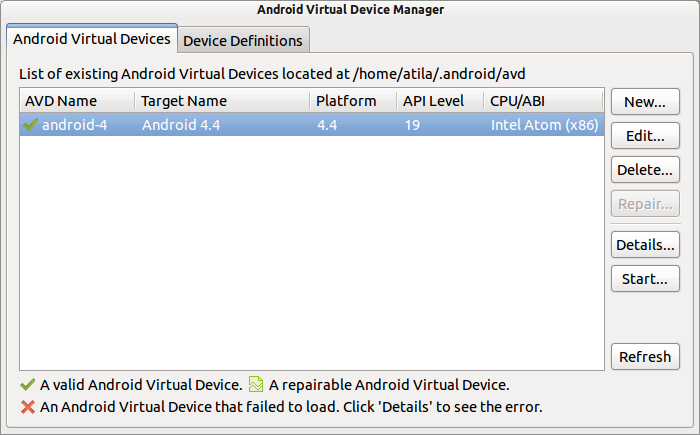
\includegraphics[scale=0.5]{img/preparando-ambiente/android-avd.png}
    \caption{Android AVD}
\end{figure}

Vamos aproveitar e criar nosso \gls{avd} para testar pela primeira vez
nosso emulador. Ainda no Android Studio clique em \texttt{Tools}
$\rightarrow$ \texttt{Android} $\rightarrow$ \texttt{AVD Manager}. Na
aba \texttt{Android Virtual Devices} clique em \texttt{New...}

Dê um nome. Você pode usar qualquer nomenclatura, mas é interessante que
tenha algo haver com a versão. Assim, caso você tenha que testar seu
código em outras versões você poderá saber qual emulador utilizar. Por
exemplo use \texttt{android-4.4}. Em \texttt{Target} escolha a versão,
neste caso \texttt{Android 4.4 (API 19)}. Pronto, apenas clique em
\texttt{Create AVD}.

\subsubsection{Dicas}

A opção \texttt{Device} indica qual a resolução da tela do aparelho.
Como não é possível redimensionar a janela, em alguns monitores a janela
fica maior que a tela do seu monitor.

A opção \texttt{Snapshot} quando habilitada, serve para salvar o estado
do emulador. Isso faz com que da segunda inicialização em diante se
torne mais rápida.

A opção \texttt{SD Card} é ideal caso sua aplicação necessite guardar
dados como fotos, arquivos. O AVD irá reservar um espaço em seu HD
permitindo assim o acesso a dados pelo emulador.

\subsubsection{Primeiro projeto Android \label{sssec:testando}}

Para criar um projeto no Android Studio selecione \texttt{File}
$\rightarrow$ \texttt{New Project...}

Dê um nome qualquer ao seu aplicativo, por exemplo
\texttt{hello.android}. Note que o Android Studio tenta dar um nome ao
seu pacote e ao diretório de arquivos a partir do nome que você digitou.
Deixe como está. Em \texttt{Target SDK} é preciso escolher qual API
vamos utilizar, em nosso caso escolha a \texttt{API 19: Android 4.4}. Em
\texttt{Minimum Required SDK} escolha a
\texttt{API 8: Android 2.2 (Froyo)} indicando que a versão mínima é a
\texttt{API 8}. Clique em \texttt{Next}.

É possível criar o ícone lançador logo ao criar o aplicativo. Selecione
da maneira que achar melhor e clique em \texttt{Next}. Em seguida temos
a tela inicial do projeto, a opção \texttt{Blank Activity} vem
selecionado por padrão, clique em \texttt{Next}. Por fim clique em
\texttt{Finish}.

Após isso basta executar o projeto usando \texttt{Shift + F10} ou no
menu \texttt{Run} $\rightarrow$ \texttt{Run 'main'}. Se tudo tiver dado
certo é possível ver no emulador sua primeira aplicação rodando.

\subsubsection{Dicas}

Uma vez que você abriu o emulador não o feche. Você irá notar que ao
abrir pela primeira vez ele leva um tempo para isso. Neste caso ao
atualizar o código-fonte apenas rode o aplicativo novamente. O plugin
ADT fará com que o aplicativo seja reinstalado no emulador.

Faça o teste com alguns atalhos básicos:

\begin{itemize}
\item
  \textbf{\texttt{Alt + Enter}} Maximiza o emulador. Ideal para
  demostrações.
\item
  \textbf{\texttt{Ctrl + F11}} Muda a orientação do emulador, retrato ou
  paisagem.
\item
  \textbf{\texttt{F8}} Liga/desliga a rede.
\end{itemize}
Para mais detalhes acesse
\url{http://developer.android.com/tools/help/emulator.html#KeyMapping}

Outro elemento essencial é o \texttt{LogCat}. Ele é responsável por
mostrar as mensagens de \emph{log} do emulador. Caso você encontre
problemas com seu código o \texttt{LogCat} será seu melhor aliado. Para
acessá-lo utilize o atalho \texttt{Alt + 6}.

\subsection{Sqlite3}

Sendo o Sqlite o banco de dados embutido na plataforma Android, nada
melhor do que aprendermos um pouco sobre ele.

O Sqlite é um banco de dados relacional bastante utilizado por
dispositivos e sistemas embarcados por ser leve, robusto, de fácil
configuração e, acima de tudo, livre. Para a instalação, abra um
terminal como \texttt{root} e:

\begin{verbatim}
$ sudo su
# apt-get install sqlite3
\end{verbatim}
Após a instalação é possível utilizar o Sqlite via linha de comando.
Faça \emph{logoff} do usuário \texttt{root} e faça os seguintes testes:

\begin{verbatim}
# exit
$ sqlite
SQLite version 2.8.17
Enter ".help" for instructions
sqlite>
\end{verbatim}
Você deverá ver algo parecido. Para sair utilize o comando
\texttt{.exit}. Veja outros detalhes na página oficial do projeto:
\url{http://www.sqlite.org/}.

\subsubsection{Tipos de dados}

Utilize a tabela abaixo para criar suas tabelas futuramente.

\ctable[caption = Tipos de dados do Sqlite, pos = H, center, botcap]{ll}
{% notes
}
{% rows
\FL
\parbox[b]{0.14\columnwidth}{\raggedright
\textbf{Nome}
} & \parbox[b]{0.86\columnwidth}{\raggedright
\textbf{Descrição}
}
\ML
\parbox[t]{0.14\columnwidth}{\raggedright
\texttt{INTEGER}
} & \parbox[t]{0.86\columnwidth}{\raggedright
valores inteiros, positivos ou negativos. Podem variar de 1 a 8
\emph{bytes}.
}
\\\noalign{\medskip}
\parbox[t]{0.14\columnwidth}{\raggedright
\texttt{REAL}
} & \parbox[t]{0.86\columnwidth}{\raggedright
valores reais ou decimais.
}
\\\noalign{\medskip}
\parbox[t]{0.14\columnwidth}{\raggedright
\texttt{TEXT}
} & \parbox[t]{0.86\columnwidth}{\raggedright
usado para armazenar valores, não-limitado. Suporta várias codificações,
por exemplo \texttt{UTF-8}.
}
\\\noalign{\medskip}
\parbox[t]{0.14\columnwidth}{\raggedright
\texttt{BLOB}
} & \parbox[t]{0.86\columnwidth}{\raggedright
objetos binários tais como imagens, arquivos de texto, etc. Também
possui tamanho não-limitado.
}
\\\noalign{\medskip}
\parbox[t]{0.14\columnwidth}{\raggedright
\texttt{NULL}
} & \parbox[t]{0.86\columnwidth}{\raggedright
representa falta de informação.
}
\LL
}

\subsection{Sqliteman}

\begin{figure}[h]
\centering
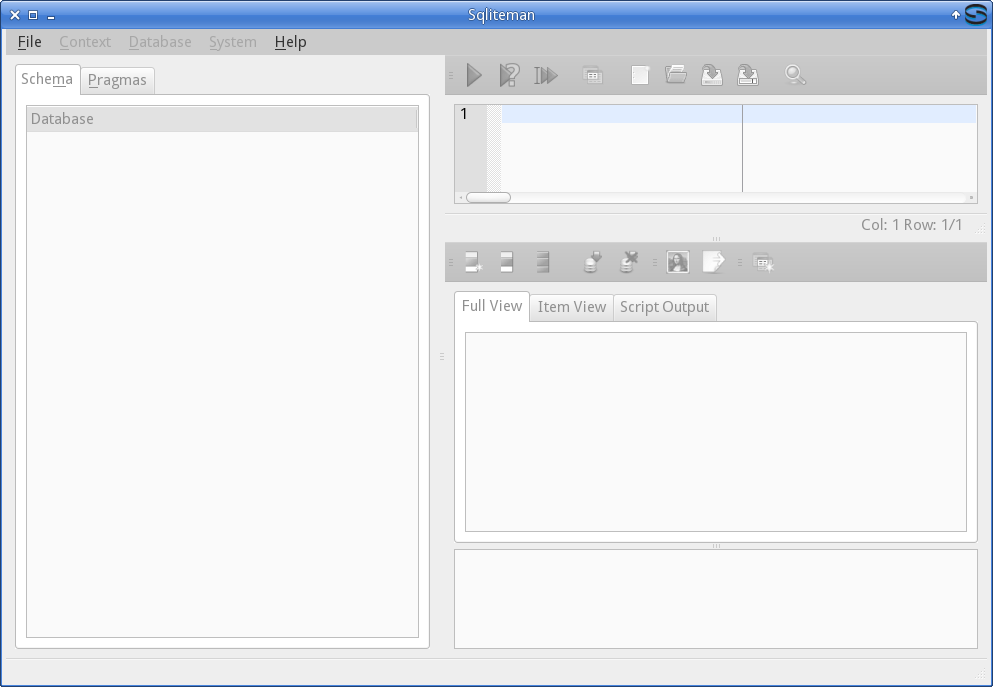
\includegraphics[scale=0.4]{img/preparando-ambiente/sqliteman.png}
\caption{Sqliteman}
\end{figure}

Para uma gerência mais produtiva usaremos o Sqliteman para acessar e
modificar bancos de dados. A instalação é feita via linha de comando.
Abra um terminal e:

\begin{verbatim}
$ sudo su
# apt-get install sqliteman
\end{verbatim}
Depois de instalado, acesse o aplicativo do menu principal do Ubuntu em
\texttt{Aplicativos} $\rightarrow$ \texttt{Escritório} $\rightarrow$
\texttt{Sqliteman}. Faça alguns testes criando bancos de dados, depois
crie algumas tabelas. Ele possui assistentes que irão auxiliar nos
primeiros momentos.

Por exemplo, crie uma base de dados e depois clique com o botão direito
do \emph{mouse} em \texttt{Tables}. Utilize o assistente e veja como é
simples criar tabelas no sqlite.

\begin{listing}[H]
  \inputminted[linenos=true,frame=bottomline,tabsize=3]{ sql }{ source/exemplo-bd-1.sql }
  \caption{Exemplo de banco de dados [exemplo-bd.sql]}
\end{listing}

Observe que podemos fazer auto-relacionamento na tabela. Assim somos
capazes de executar a seguinte SQL, contando o número de distros que
derivam de uma outra original. Veja:

\begin{listing}[H]
  \inputminted[linenos=true,frame=bottomline,tabsize=3]{ sql }{ source/exemplo-bd-2.sql }
  \caption{Exemplo de \textit{query} com \textit{subquery} [exemplo-bd.sql]}
\end{listing}

Mais informações em: \url{http://sqliteman.com/}

\subsection{Inkscape}

\begin{figure}[h]
\centering
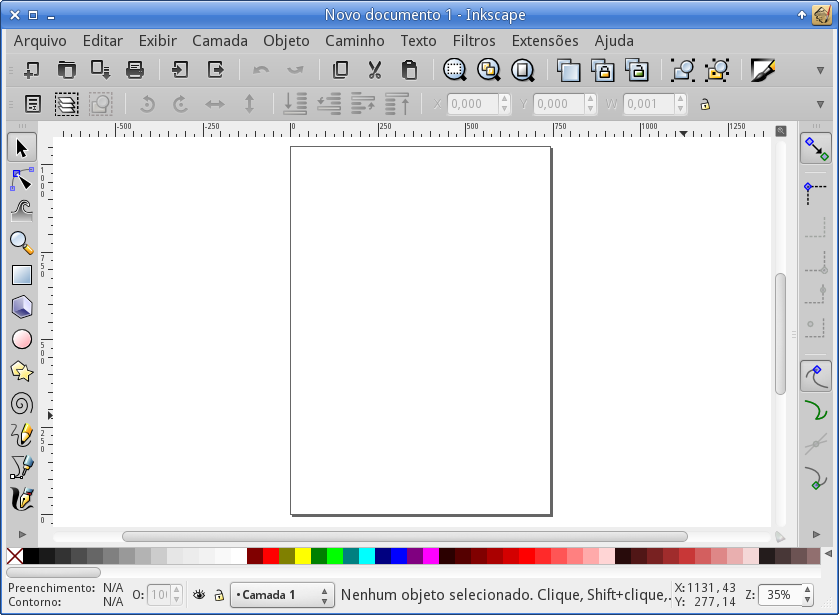
\includegraphics[scale=0.45]{img/preparando-ambiente/inkscape.png}
\caption{Inkscape}
\end{figure}

Uma ótima ferramenta de desenho vetorial é o Inkscape. Ela será bastante
útil pois o desenvolvimento de aplicativos hoje em dia é baseado muito
em figuras para facilitar a navegação, identidade visual, entre outras
coisas.

A instalação é feita de forma simples. Num terminal:

\begin{verbatim}
$ sudo su
# apt-get install inkscape
\end{verbatim}
Para dicas de como criar ícones para os diversos elementos do Android
veja a página
\url{http://developer.android.com/design/style/iconography.html}.

\begin{figure}[h]
    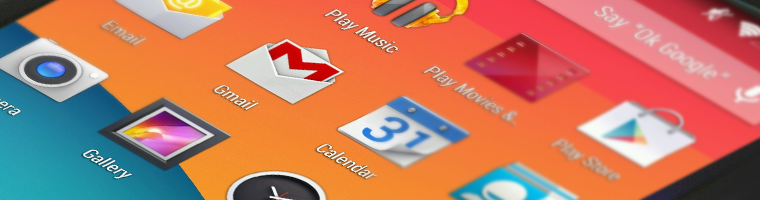
\includegraphics[scale=0.5]{img/preparando-ambiente/iconography-overview.png}
    \caption{Visão geral da iconografia do Android}
\end{figure}


\chapter{Exemplo prático}

\section{Primeira aplicação - Contatos}

Baseado em \ref{sssec:testando} Testando o ADT, crie um novo aplicativo
chamado \textbf{Contatos}. Use \texttt{guia.android.exemplo} como o nome
da companhia. Siga os passos descritos nas figuras
\ref{fig:new-project-1}, \ref{fig:new-project-2},
\ref{fig:new-project-3} e \ref{fig:new-project-4} para criar uma
\texttt{Activity} inicial chamada \texttt{MainActivity} e um
\emph{layout} inicial chamado \texttt{main}. Depois clique em
\texttt{Finish}.

\begin{figure}[h]
    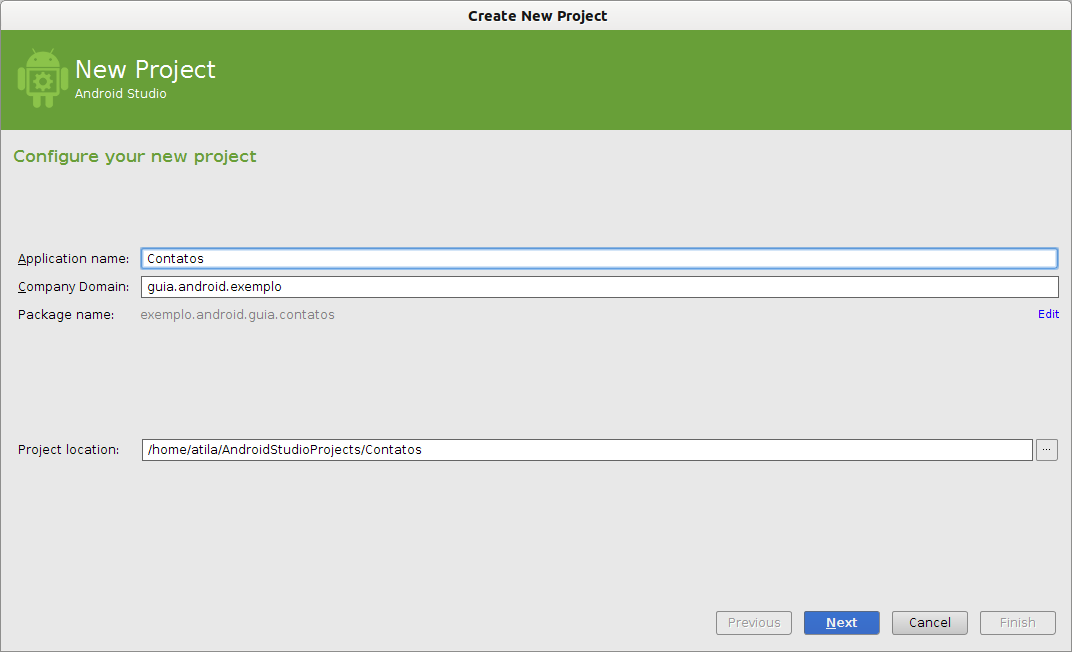
\includegraphics[scale=0.35]{img/exemplo-pratico/android-new-project-1.png}
    \caption{Novo projeto, tela 1}
    \label{fig:new-project-1}
\end{figure}

\begin{figure}[p]
    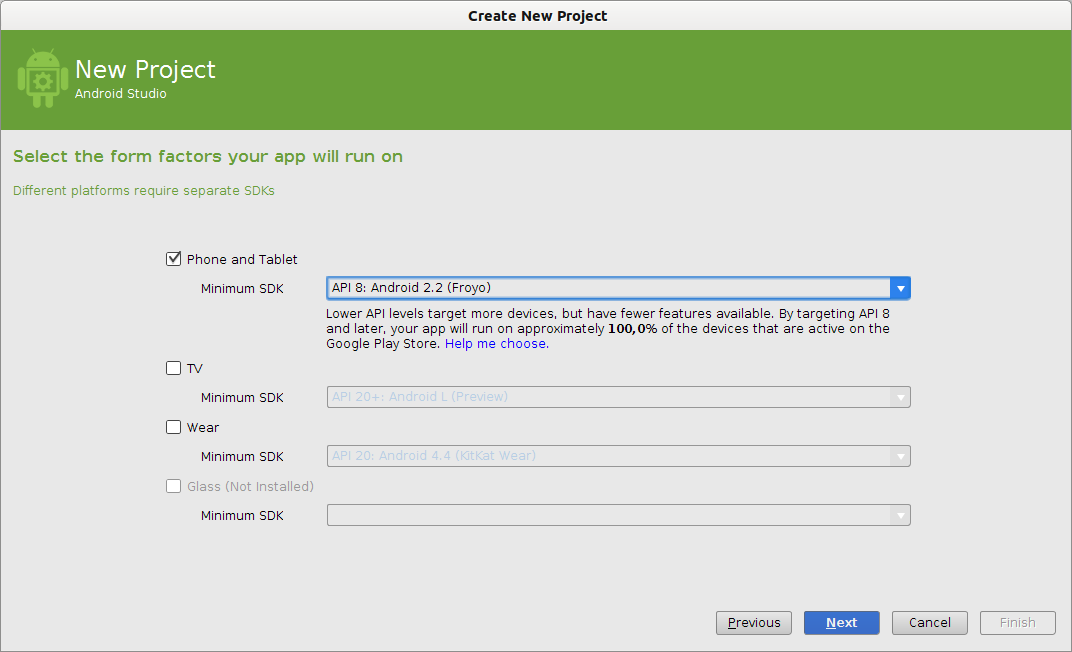
\includegraphics[scale=0.35]{img/exemplo-pratico/android-new-project-2.png}
    \caption{Novo projeto, tela 2}
    \label{fig:new-project-2}
\end{figure}

\begin{figure}[p]
    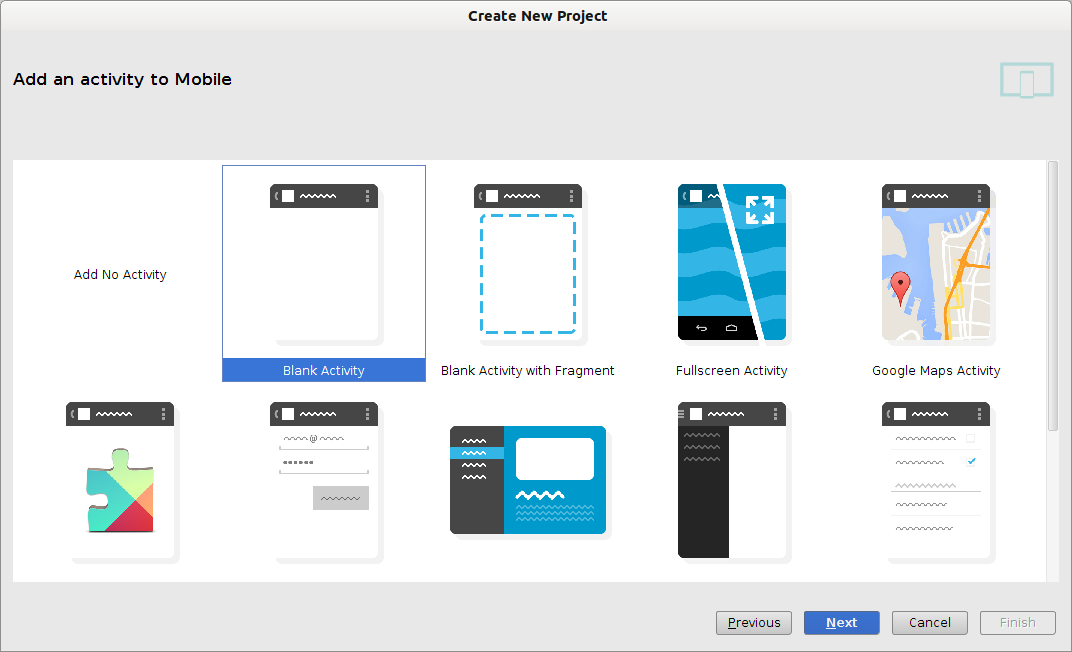
\includegraphics[scale=0.35]{img/exemplo-pratico/android-new-project-3.png}
    \caption{Novo projeto, tela 3}
    \label{fig:new-project-3}
\end{figure}

\begin{figure}[h]
    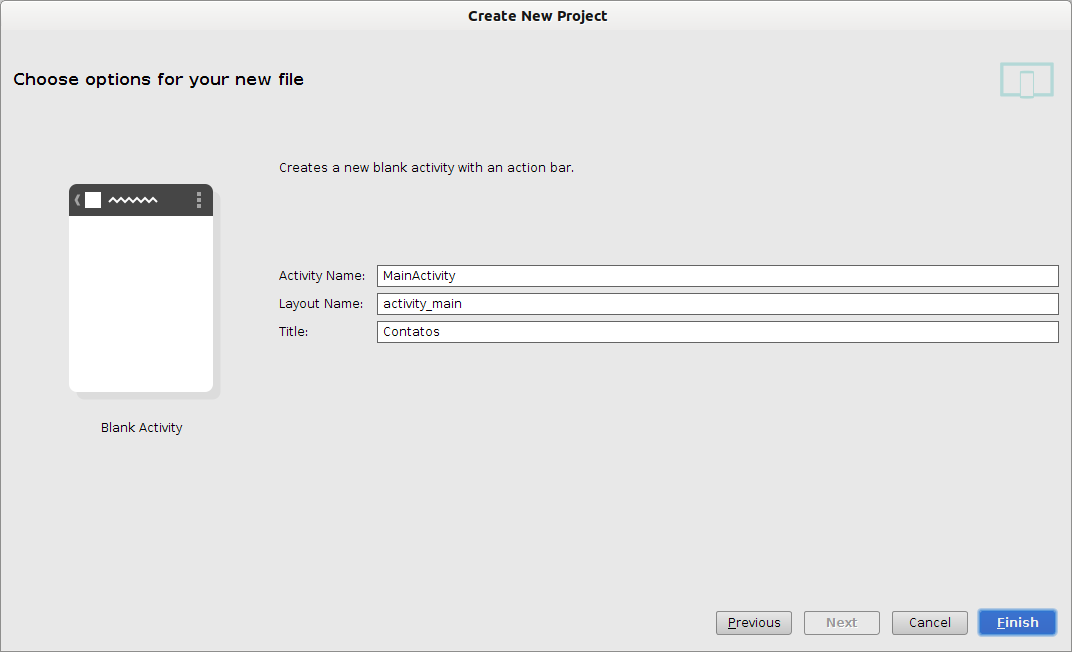
\includegraphics[scale=0.32]{img/exemplo-pratico/android-new-project-4.png}
    \caption{Novo projeto, tela 4}
    \label{fig:new-project-4}
\end{figure}

Este exemplo é bastante útil para aprendermos como funciona o Android.
Você só poderá criar algo se você souber utilizar bem as ferramentas.

\subsection{AndroidManifest.xml}

Este é o arquivo que define nossa aplicação, mapeia as
\texttt{Activity}'s, entre outras configurações. Ao finalizar a criação
do projeto, inicialmente este arquivo deverá conter o conteúdo descrito
no Código-fonte \ref{code:android-manifest-1}:

\begin{listing}[H]
  \inputminted[linenos=true,frame=bottomline,tabsize=3]{ xml }{ source/AndroidManifest-1.xml }
  \caption{Projeto inicial [AndroidManifest.xml]}
  \label{code:android-manifest-1}
\end{listing}

Devido a entrada do \gls{gradle} (ver
\href{http://www.gradleware.com/android/gradle-the-new-android-build-system/}{Gradle:
The New Android Build System}) a versão mínima e a versão alvo do SDK
foram movidas para o arquivo \texttt{build.gradle}. Outros detalhes em
\url{http://developer.android.com/sdk/installing/studio-build.html}.

\subsubsection{Links para ver o código online}

Desse ponto em diante você verá a cada código mostrado um link para o
código online, no \gls{github}. Se você está na versão eletrônica basta
clicar no link. Se você está na versão impressa acesse a página web
\url{https://github.com/atilacamurca/guia-aberto-android-contatos/commits/master}.

\subsubsection{Commit}

\href{https://github.com/atilacamurca/guia-aberto-android-contatos/commit/d47028c8b7273f5a10c849c8b487f262360ded56}{d47028c8b7273f5a10c849c8b487f262360ded56}

\subsection{Activity \label{ssec:act}}

Não existe método \texttt{main} visível ao programador no Android. Ao
invés disso temos \texttt{Activity}'s. Para que o Android saiba qual ele
deve iniciar primeiro utilizamos um \texttt{intent-filter} como visto no
trecho de código acima da linha \circled{09} a \circled{12}. Para nossa
primeira \texttt{Activity} criaremos uma lista de contatos e um menu
para criação de um novo contato.

Para construir o \emph{layout} inicial de nossa aplicação precisamos
editar o arquivo \texttt{activity\_main.xml} localizado em
\texttt{res/layout}.

\begin{listing}[H]
  \inputminted[linenos=true,frame=bottomline,tabsize=3]{ xml }{ source/main-1.xml }
  \caption{Layout principal [res/layout/activity_main.xml]}
\end{listing}

O resultado pode ser visto na figura \ref{fig:activity-main-1}.

\begin{figure}[h]
    \center
    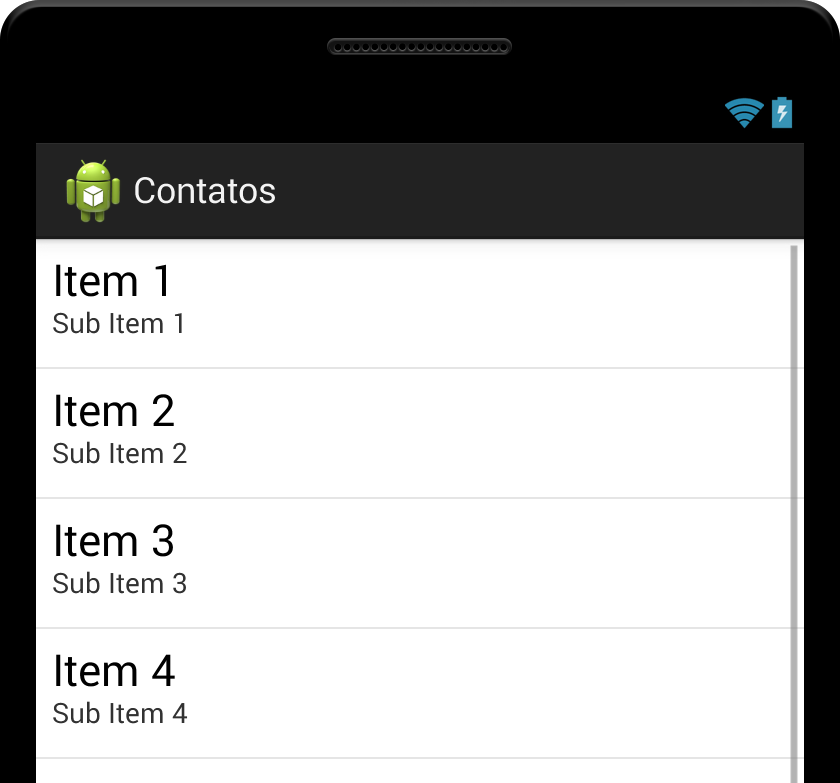
\includegraphics[scale=0.3]{img/exemplo-pratico/activity_main-1.png}
    \caption{Layout tela principal}
    \label{fig:activity-main-1}
\end{figure}

\subsubsection{Commit}

\href{https://github.com/atilacamurca/guia-aberto-android-contatos/commit/5e31fe9e7c9b15596ae6bfe1ca857d92544290a2}{5e31fe9e7c9b15596ae6bfe1ca857d92544290a2}

Deste momento em diante tenha em mente que os arquivos \gls{xml} aqui
descritos são apenas para você poder comparar e ver se não esqueceu de
nada. Todos os \emph{layout}'s devem ser criados usando o
\gls{layout-editor}. Você irá notar que ao abrir o \texttt{xml} uma
janela de \emph{layout} aparecerá. Para visualizar o \texttt{xml} ou o
\emph{layout} gráfico basta utilizar a aba inferior esquerda.

Por fim, temos o menu. Clique com o botão direito do \emph{mouse} no
diretório \texttt{res/menu} $\rightarrow$ \texttt{New} $\rightarrow$
\texttt{Menu resource file}. Chame-o de \texttt{main\_menu.xml}.

\begin{listing}[H]
  \inputminted[linenos=true,frame=bottomline,tabsize=3]{ xml }{ source/main_menu-1.xml }
  \caption{Menu principal [res/menu/main\b{ }menu.xml]}
\end{listing}

\subsubsection{Commit}

\href{https://github.com/atilacamurca/guia-aberto-android-contatos/commit/a49787ebc586dca2db9fa3adc92b134453258354}{a49787ebc586dca2db9fa3adc92b134453258354}

\begin{figure}[h]
    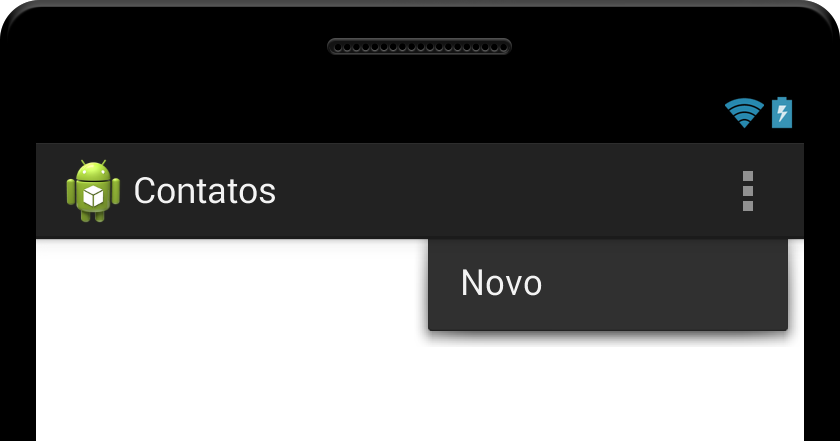
\includegraphics[scale=0.3]{img/exemplo-pratico/main_menu-1.png}
    \caption{Menu principal}
\end{figure}

Pronto, já temos nosso layout. Compile o projeto e vamos a próxima
iteração.

\subsubsection{Convenção de nomes para ícones \label{sssec:nomeicones}}

Na edição 2 deste guia, falamos sobre o uso de ícones no menu e seus
\emph{namespaces}. Mas desde a versão 3.0, o Android introduziu o
conceito de \textbf{Action Bar}. Isso fez com que o uso de ícones no
menu sumisse.

\begin{itemize}
\item
  \url{http://android-developers.blogspot.in/2012/01/say-goodbye-to-menu-button.html}
\item
  \url{http://developer.android.com/guide/topics/ui/actionbar.html}
\end{itemize}
Mesmo assim vou manter a tabela com as convenções adotadas pelo Android
para o prefixo dos ícones:

\ctable[caption = Convenção para nome dos ícones,
pos = H, center, botcap]{lll}
{% notes
}
{% rows
\FL
\parbox[b]{0.29\columnwidth}{\raggedright
\textbf{Tipo de Recurso}
} & \parbox[b]{0.26\columnwidth}{\raggedright
\textbf{Prefixo}
} & \parbox[b]{0.43\columnwidth}{\raggedright
\textbf{Exemplo}
}
\ML
\parbox[t]{0.29\columnwidth}{\raggedright
Ícones
} & \parbox[t]{0.26\columnwidth}{\raggedright
\texttt{ic\_}
} & \parbox[t]{0.43\columnwidth}{\raggedright
\texttt{ic\_adicionar.png}
}
\\\noalign{\medskip}
\parbox[t]{0.29\columnwidth}{\raggedright
Launcher icons
} & \parbox[t]{0.26\columnwidth}{\raggedright
\texttt{ic\_launcher\_}
} & \parbox[t]{0.43\columnwidth}{\raggedright
\texttt{ic\_launcher\_calendario.png}
}
\\\noalign{\medskip}
\parbox[t]{0.29\columnwidth}{\raggedright
Menu e Action Bar
} & \parbox[t]{0.26\columnwidth}{\raggedright
\texttt{ic\_menu\_}
} & \parbox[t]{0.43\columnwidth}{\raggedright
\texttt{ic\_menu\_ajuda.png}
}
\\\noalign{\medskip}
\parbox[t]{0.29\columnwidth}{\raggedright
Status bar icons
} & \parbox[t]{0.26\columnwidth}{\raggedright
\texttt{ic\_stat\_notify\_}
} & \parbox[t]{0.43\columnwidth}{\raggedright
\texttt{ic\_stat\_notify\_msg.png}
}
\\\noalign{\medskip}
\parbox[t]{0.29\columnwidth}{\raggedright
Tab icons
} & \parbox[t]{0.26\columnwidth}{\raggedright
\texttt{ic\_tab\_}
} & \parbox[t]{0.43\columnwidth}{\raggedright
\texttt{ic\_tab\_recente.png}
}
\\\noalign{\medskip}
\parbox[t]{0.29\columnwidth}{\raggedright
Dialog icons
} & \parbox[t]{0.26\columnwidth}{\raggedright
\texttt{ic\_dialog\_}
} & \parbox[t]{0.43\columnwidth}{\raggedright
\texttt{ic\_dialog\_info.png}
}
\LL
}

Note que você não é obrigado a utilizar os prefixos citados acima, isto
é apenas uma convenção. Veja mais detalhes em
\url{http://developer.android.com/design/style/iconography.html#action-bar}.

Abra o arquivo \texttt{MainActivity.java} e vá ao método
\texttt{onCreate}. Defina o \emph{layout} como sendo nosso
\texttt{main.xml}. Para isso adicione o \emph{layout} \textbf{main} ao
final do método:

\begin{listing}[H]
  \inputminted[linenos=true,frame=bottomline,tabsize=3]{ java }{ source/MainActivity-1.java }
  \caption{Definir layout [MainActivity.java]}
\end{listing}

\subsubsection{Commit}

\href{https://github.com/atilacamurca/guia-aberto-android-contatos/commit/a49787ebc586dca2db9fa3adc92b134453258354}{a49787ebc586dca2db9fa3adc92b134453258354}

\paragraph{Cuidado \label{par:r}}

no ambiente Android temos uma classe chamada \texttt{R}. Ela existe
tanto na biblioteca do Android como em cada projeto. A classe
\texttt{android.R} é utilizada em outras situações, onde códigos
pré-prontos foram disponibilizados pela equipe do Android.

Agora precisamos sobrescrever os métodos \texttt{onCreateOptionsMenu} e
\texttt{onOptionsItemSelected}. Eles irão criar o menu a partir de nosso
\emph{layout} e notificar quando os itens do menu forem pressionados,
respectivamente. Vamos ao código:

\begin{listing}[H]
  \inputminted[linenos=true,frame=bottomline,tabsize=3]{ java }{ source/MainActivity-2.java }
  \caption{Criando o menu [MainActivity.java]}
\end{listing}

\subsubsection{Commit}

\href{https://github.com/atilacamurca/guia-aberto-android-contatos/commit/18c59c4a828c40f0877f0adef352b1afe6c3412f}{18c59c4a828c40f0877f0adef352b1afe6c3412f}

\subsection{Formulários}

Agora vamos criar nosso formulário para criação e edição de contatos.
Começaremos pelo \emph{layout}. Crie um arquivo \texttt{xml} em
\texttt{res/layout} chamado \texttt{activity\_salvar.xml}.

Existem alguns pontos importantes para este trecho de código. Começando
pelo \emph{layout} inicial, onde usaremos \texttt{TableLayout} (dentro
de um \texttt{RelativeLayout}). Esse \emph{layout} é ideal para telas
com estilo tabela.

\begin{figure}[h]
    \center
    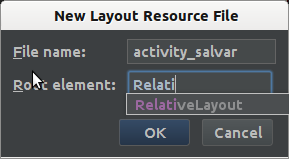
\includegraphics[scale=0.6]{img/exemplo-pratico/new-layout-salvar.png}
    \caption{Novo layout, Root element com busca de layouts disponíveis}
\end{figure}

Um detalhe importante para observarmos neste \emph{layout} é que ele
possui o atributo \texttt{stretchColumns} com valor \texttt{1}. Isso
quer dizer que a coluna \texttt{1} da tabela terá o maior tamanho
possível, respeitando o tamanho mínimo das outras células. Para
visualizar as mudanças você pode tentar usar outros valores como
\texttt{0} tornando a primeira coluna maior que as demais, ou ainda
\texttt{*} que fará com que todas as células tenham o mesmo tamanho.

\begin{listing}[H]
  \inputminted[linenos=true,frame=bottomline,tabsize=3]{ xml }{ source/activity_salvar-1.xml }
  \caption{Formulário principal [res/layout/activity_salvar.xml]}
\end{listing}

\subsubsection{Commit}

\href{https://github.com/atilacamurca/guia-aberto-android-contatos/commit/f130f18bcdab8638641d42c32557ffffa2e1b0ba}{f130f18bcdab8638641d42c32557ffffa2e1b0ba}

\bigskip

Atentem para a linha \circled{23} do código acima. Nele podemos ver o
uso do indicador do tipo de dados que vamos entrar, no caso
\texttt{textPersonName}. Isso significa que o teclado irá se comportar
de forma a ajudar o usuário, fazendo com que a primeira letra seja
digitada sempre em maiúsculo. Sabendo disso use o mesmo raciocínio para
os campos Telefone e E-mail, usando o valor \texttt{phone} e
\texttt{textEmailAddress} em \texttt{android:inputType},
respectivamente.

A lista completa pode ser vista em
\url{http://developer.android.com/reference/android/widget/TextView.html#attr_android:inputType}.

\begin{figure}[H]
    \center
    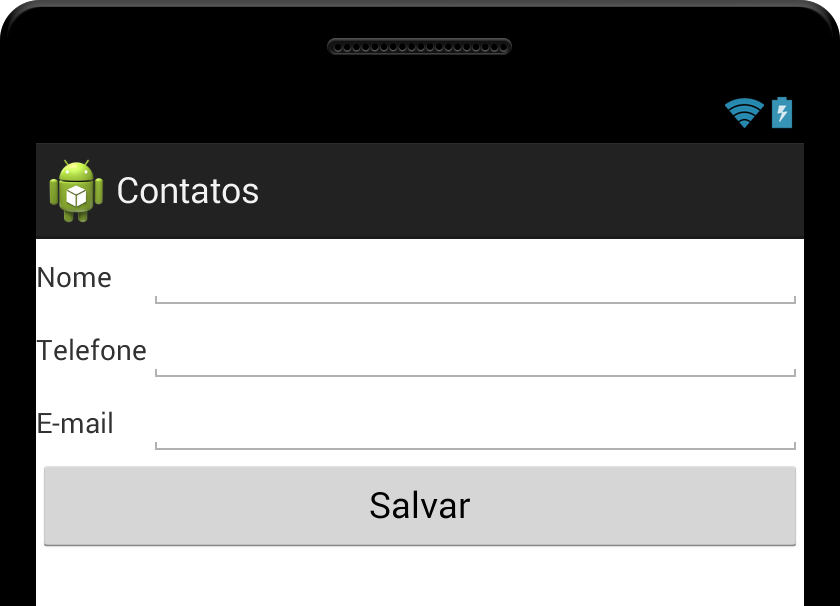
\includegraphics[scale=0.3]{img/exemplo-pratico/activity_salvar-1.png}
    \caption{Layout tela Salvar Contato}
\end{figure}

Crie uma nova \texttt{Activity} chamada \texttt{SalvarActivity} dentro
de \texttt{contatos.app.view}. Para irmos de uma \texttt{Activity} para
outra precisamos de um \texttt{Intent}. Um de seus construtores recebe
como parâmetros a instância da classe em que estamos, sendo que ela deve
implementar a interface \texttt{Context} e o nome da classe a qual deve
ser mostrada. Veja como implementar o método \texttt{irParaSalvar} da
classe \texttt{MainActivity}:

\begin{listing}[H]
  \inputminted[linenos=true,frame=bottomline,tabsize=3]{ java }{ source/MainActivity-3.java }
  \caption{Mudando de Activity [MainActivity.java]}
\end{listing}

\subsubsection{Commit}

\href{https://github.com/atilacamurca/guia-aberto-android-contatos/commit/ec5b0f1913e300a91bde424f596cc15e25b9ef18}{ec5b0f1913e300a91bde424f596cc15e25b9ef18}

\medskip

Veremos agora como manipular \texttt{EditText}'s, que representam os
campos de entrada de dados. Abra o \texttt{SalvarActivity} e adicione o
método carregar e crie atributos para guardar os \texttt{EditText}'s:

\begin{listing}[H]
  \inputminted[linenos=true,frame=bottomline,tabsize=3]{ java }{ source/SalvarActivity-1.java }
  \caption{Utilizando EditText's [SalvarActivity.java]}
\end{listing}

\subsubsection{Commit}

\href{https://github.com/atilacamurca/guia-aberto-android-contatos/commit/16671ee3a0afeec91431deb656aeaab906d4abb8}{16671ee3a0afeec91431deb656aeaab906d4abb8}

\bigskip

Para que a \texttt{Activity} funcione precisamos mapeá-la no arquivo
\texttt{AndroidManifest.xml}. Adicione o conteúdo abaixo entre as
\emph{tags} \texttt{application}:

\begin{listing}[H]
  \inputminted[linenos=true,frame=bottomline,tabsize=3]{ xml }{ source/AndroidManifest-2.xml }
  \caption{Mapear SalvarActivity [AndroidManifest.xml]}
\end{listing}

\subsubsection{Commit}

\href{https://github.com/atilacamurca/guia-aberto-android-contatos/commit/fb4b54a586e6669ab4974cbf7d38edb5b72eb1a4}{fb4b54a586e6669ab4974cbf7d38edb5b72eb1a4}

\subsection{Construindo o Model da aplicação \label{ssec:model}}

Precisamos de um \emph{helper} para fazer acesso ao banco de dados. O
Android provê suporte a bancos de dados
\href{http://sqlite.org/}{Sqlite} por padrão. Qualquer banco de dados
que você criar será acessível pelo nome por qualquer classe na sua
aplicação, mas não fora dela.

Crie uma classe chamada \texttt{ContatoHelper} em
\texttt{contatos.app.model} que extende de \texttt{SQLiteOpenHelper}.
Essa classe será capaz de ler e escrever no banco de dados graças aos
métodos \texttt{getReadableDatabase()} e \texttt{getWritableDatabase()},
respectivamente.

A princípio temos que criar um construtor passando como parâmetros o
nome do banco de dados e a versão da \gls{ddl} (\emph{Data Definition
Language}). Logo em seguida precisamos implementar os métodos
\texttt{onCreate}, no qual iremos criar as tabelas e \texttt{onUpdate},
caso tenhamos que alterar alguma tabela em versões futuras do
aplicativo.

\begin{listing}[H]
  \inputminted[linenos=true,frame=bottomline,tabsize=3]{ java }{ source/ContatoHelper-1.java }
  \caption{Helper da aplicação [ContatoHelper.java]}
\end{listing}

Para a iteração de criação de um novo contato, ainda em
\texttt{ContatoHelper} vamos adicionar um método \texttt{criar}. Faça:

\begin{listing}[H]
  \inputminted[linenos=true,frame=bottomline,tabsize=3]{ java }{ source/ContatoHelper-2.java }
  \caption{Criar novo contato [ContatoHelper.java]}
\end{listing}

Agora temos que fazer a chamada do método criar da classe
\texttt{ContatoHelper} em \texttt{SalvarActivity}. Para isso temos que
criar uma instância de \texttt{ContatoHelper}, adicionar o botão salvar
e adicionar um \emph{Listener} de \emph{click} (faça o \emph{import} da
classe \newline
\texttt{android.view.View.OnClickListener}). Vamos ao código:

\begin{listing}[H]
  \inputminted[linenos=true,frame=bottomline,tabsize=3]{ java }{ source/SalvarActivity-2.java }
  \caption{Fim da iteração criar contato [SalvarActivity.java]}
\end{listing}

Com essa implementação já é possível salvar contatos na base de dados.

\subsection{Mostrando os dados na View \label{ssec:listview}}

Após salvar os dados no banco, devemos ser capazes de obter tais
informações e colocá-las em forma de Lista. Para isso criaremos um novo
\emph{layout} que será responsável por representar uma linha de nossa
Lista. Essa linha deve ser semelhante a figura abaixo:

\begin{figure}[h]
    \centering
    \includegraphics[scale=0.6]{img/layout-linha.png}
    \caption{Layout linha da Lista}
\end{figure}

Para isso crie um arquivo chamado \texttt{linha.xml} em
\texttt{res/layout} com o seguinte conteúdo.

\begin{listing}[H]
  \inputminted[linenos=true,frame=bottomline,tabsize=3]{ xml }{ source/linha-1.xml }
  \caption{Layout para cada linha da lista [res/layout/linha.xml]}
\end{listing}

Note a possibilidade de aninhar o \texttt{LinearLayout}. Fazendo isso é
possível criar o \emph{layout} desejado fazendo com que alguns elementos
sejam inseridos na horizontal, outros na vertical.

Outro ponto interessante é o uso de negrito no \texttt{TextView}
correspondente ao nome, na linha \circled{14}, e o uso de reticências
caso o nome seja maior que a tela usando
\texttt{android:ellipsize="end"} na linha \circled{15}.

Agora vamos até \texttt{ContatoHelper} e adicionar o método
\texttt{listar}. E também adicionaremos métodos para facilitar a
obtenção dos valores de cada atributo.

\begin{listing}[H]
  \inputminted[linenos=true,frame=bottomline,tabsize=3]{ java }{ source/ContatoHelper-3.java }
  \caption{Listar contatos existentes [ContatoHelper.java]}
\end{listing}

Os elementos de um \texttt{Cursor} são numerados iniciando de 0 (zero).
Neste caso o 0 é a coluna \texttt{\_id}. Observe que ela não será usada
pelo programador e sim pelo Android. Isto será visto com mais detalhes
em \ref{ssec:edit} Editando dados existentes.

Para popular cada linha de nossa Lista vamos criar uma classe interna
(\emph{inner class}) em \texttt{MainActivity}. Assim podemos fazer
\emph{cache} dos objetos aumentando a performance. Use o sufixo
\texttt{Holder} para esse tipo de classe.

\begin{listing}[H]
  \inputminted[linenos=true,frame=bottomline,tabsize=3]{ java }{ source/MainActivity-4.java }
  \caption{Classe Holder [MainActivity.java]}
\end{listing}

Levando em conta que estamos usando a interface \texttt{Cursor} em nosso
\texttt{Helper} temos que criar uma classe que extenda de
\texttt{CursorAdapter} que será responsável por definir o \emph{layout}
de cada linha da Lista. Crie uma classe interna chamada
\texttt{ContatoAdapter}. Iremos sobrescrever dois métodos,
\texttt{newView()} e \texttt{bindView()}, que são responsáveis por
inflar (\emph{inflate}) uma nova linha e reciclar uma linha existente,
respectivamente.

\begin{listing}[H]
  \inputminted[linenos=true,frame=bottomline,tabsize=3]{ java }{ source/MainActivity-5.java }
  \caption{Classe Adapter [MainActivity.java]}
\end{listing}

Com a introdução do \texttt{Helper} teremos que criar uma instância da
classe \texttt{Cursor} para popular nossa \texttt{ListView}. Vamos ao
código-fonte:

\begin{listing}[H]
  \inputminted[linenos=true,frame=bottomline,tabsize=3]{ java }{ source/MainActivity-6.java }
  \caption{Popular ListView [MainActivity.java]}
\end{listing}

Nunca esquecendo de fechar o \texttt{helper} ao sair, pois assim
garantimos que a conexão com o banco será fechada.

\subsection{Editando dados existentes \label{ssec:edit}}

Para a edição de informações usaremos o mesmo \texttt{Activity} que
usamos para criar um contato, ou seja, \texttt{SalvarActivity}. Mas para
isso precisamos passar um parâmetro para o \texttt{Activity}. Usaremos
então um método do \texttt{Intent} que é responsável por isso,
\texttt{putExtra(chave, valor)}.

Para uma passagem de parâmetros segura devemos usar um \emph{namespace}
para que não colida com nenhum nome já utilizado pelo Android. Assim,
vamos criar uma variável estática do tipo \texttt{String}. Isso
acontecerá quando o usuário pressionar a linha que ele deseja editar.
Podemos fazer isso utilizando a interface \texttt{OnItemClickListener}.

Vamos incrementar também o método \texttt{irParaSalvar} passando o
parâmetro caso haja um. Vamos ao código:

\begin{listing}[H]
  \inputminted[linenos=true,frame=bottomline,tabsize=3]{ java }{ source/MainActivity-7.java }
  \caption{Passagem de parâmetros [MainActivity.java]}
\end{listing}

Agora é hora de tratar nosso parâmetro no \texttt{SalvarActivity}. Caso
haja um parâmetro precisamos obter os dados existentes no banco de dados
para então editá-lo. Neste caso precisaremos de mais dois métodos em
\texttt{ContatoHelper}, que são \texttt{ler} e \texttt{atualizar}.

\begin{listing}[H]
  \inputminted[linenos=true,frame=bottomline,tabsize=3]{ java }{ source/ContatoHelper-4.java }
  \caption{Ler e atualizar dados existentes [ContatoHelper.java]}
\end{listing}

O próximo passo é tratar no \texttt{SalvarActivity} caso o parâmetro
tenha sido enviado ou não. Caso positivo devemos carregar os dados
existentes no banco de dados e depois atualizá-los.

\begin{listing}[H]
  \inputminted[linenos=true,frame=bottomline,tabsize=3]{ java }{ source/SalvarActivity-3.java }
  \caption{Usando Activity para criar ou atualizar [SalvarActivity.java]}
\end{listing}

Com isso encerramos um \textbf{CRUD} básico, mas completo. A seguir
temos implementações mais específicas que irão tornar nossa aplicação
mais profissional.


\chapter{Livro de Receitas}

\section{Mostrando Diálogos}

No Android, podemos criar diálogos no \texttt{Activity} mostrando opções
ao usuário, como por exemplo, escolher itens de uma lista, ou responder
sim ou não a uma ação, etc.

Vamos incrementar algumas partes de nosso código e tentar encaixar
algumas funcionalidades relacionadas.

\subsection{Editar/Excluir ao clicar e segurar na ListView}

Vamos implementar uma ação comum no mundo Android, que é a seguinte: ao
clicar e segurar num item da \texttt{ListView}, ele mostra opções editar
e excluir, por exemplo. Isto pode ser feito facilmente usando
\texttt{AlertDialog.Builder}, uma classe com métodos pré-prontos para
serem usados por você.

Neste exemplo, precisaremos editar \texttt{ContatoHelper} e adicionar um
método para deletar um contato, editar nosso \texttt{MainActivity} no
método configurar e adicionar um \emph{Listener} que ao clicar e segurar
num item da \texttt{ListView} um método é acionado. Vamos a
implementação:

\begin{listing}[H]
  \inputminted[linenos=true,frame=bottomline,tabsize=3]{ java }{ source/ContatoHelper-5.java }
  \caption{Deletar dados existentes [ContatoHelper.java]}
\end{listing}

\begin{listing}[H]
  \inputminted[linenos=true,frame=bottomline,tabsize=3]{ java }{ source/MainActivity-8.java }
  \caption{Adicionar Listener para click longo [MainActivity.java]}
\end{listing}

Note a necessidade de um novo método em \texttt{MainActivity}, o
exibirMensagem. Ele é bastante útil quando se quer exibir uma mensagem
rapidamente e depois ela suma. Para isso usamos a classe \texttt{Toast}.

\subsubsection{Interface como parâmetro de um método}

Você já deve ter notado o uso de \emph{interface}'s como parâmetro dos
métodos, por exemplo na linha \circled{4} e \circled{11} do código
acima. Essa prática obriga ao programador implementar a classe na
passagem dos parâmetros.

Essa ideia vem de algumas linguagens de programação que possuem funções
como parâmetros para outras funções. Como o Java não suporta essa
característica, a solução veio em forma de uma \emph{interface}, a qual
o programador é obrigado a implementar seus métodos. Com isso o método
que recebe a \emph{interface} como parâmetro sabe exatamente o que ela
tem disponível.

A partir dessa observação, podemos justificar o uso da palavra reservada
final em alguns parâmetros dos métodos acima. Isso acontece porque
alguns parâmetros são utilizados dentro da implementação das
\emph{interface}'s.

Caso haja a necessidade de utilizar uma implementação em outra classe
você pode criar uma classe que implementa uma \emph{interface}, por
exemplo a \emph{interface} \texttt{OnItemLongClickListener}. Daí para a
passagem do parâmetro apenas crie uma instância da classe. Por exemplo,
suponha que você tenha uma classe chamada \texttt{OpcoesContato} que
implementa \texttt{OnItemLongClickListener}, nesse caso a linha
\circled{4} se tornaria:

\texttt{listView.setOnItemLongClickListener(new OpcoesContato());}

\subsection{Diálogo de confirmação}

Deletar dados é uma ação que deve ser feita com cuidado, então sempre é
bom confirmar com o usuário se ele deseja realmente deletar, no nosso
caso, um contato. Para isso usaremos o \texttt{AlertDialog.Builder} mais
uma vez, agora apenas com uma mensagem e os botões \emph{Sim} ou
\emph{Não}.

Ainda em \texttt{MainActivity} criaremos um outro
\texttt{AlertDialog.Builder} no momento que o usuário clicar em
\texttt{Deletar}. Segue o trecho:

\begin{listing}[H]
  \inputminted[linenos=true,frame=bottomline,tabsize=3]{ java }{ source/MainActivity-9.java }
  \caption{Diálogo de confirmação ao deletar contato [MainActivity.java]}
\end{listing}

Pronto, agora o trecho que deleta o contato foi movido para dentro do
\emph{Listener} do botão \emph{Sim}. No botão \emph{Não} passamos
\texttt{null} no \emph{Listener}, pois caso seja a opção escolhida
apenas fazemos nada. Você pode, se quiser, criar um \emph{Listener} e
mostrar uma mensagem do tipo, \emph{Cancelado pelo usuário}, para isso
usando o método \texttt{exibirMensagem}.

\subsection{Entrada de diferentes tipos de dados}

O Android foi desenvolvido com muitos recursos pré-prontos para
facilitar o desenvolvimento de aplicações. Um recurso bastante útil é a
distinção dos dados que irão ser inseridos nos \texttt{TextView}'s. Com
isso o teclado virtual do cliente se adapta ao tipo de dado que será
inserido. No nosso caso faremos distinção do campo \texttt{telefone},
onde apenas números e hífens (-) podem ser inseridos, e o campo
\texttt{e-mail} onde a presença do arroba (@) e pontos (.) são elementos
essenciais.

Vejamos alguns valores aceitos pelo \texttt{inputType}:

\begin{itemize}
\item
  Para textos:
  \begin{itemize}
  \item
    \texttt{text}
  \item
    \texttt{textCapCharacters}
  \item
    \texttt{textMultiLine}
  \item
    \texttt{textUri}
  \item
    \texttt{textEmailAddress}
  \item
    \texttt{textPersonName}
  \item
    \texttt{textPassword}
  \item
    \texttt{textVisiblePassword}
  \end{itemize}
\item
  Para números:
  \begin{itemize}
  \item
    \texttt{number}
  \item
    \texttt{numberSigned}
  \item
    \texttt{numberDecimal}
  \item
    \texttt{phone}
  \item
    \texttt{datetime}
  \item
    \texttt{date}
  \item
    \texttt{time}
  \end{itemize}
\end{itemize}
Precisaremos alterar apenas o \texttt{salvar.xml} localizado em
\texttt{res/layout}. Localize o atributo \texttt{inputType} dos campos
\texttt{telefone} e \texttt{e-mail} e altere os valores da seguinte
maneira:

\begin{listing}[H]
  \inputminted[linenos=true,frame=bottomline,tabsize=3]{ xml }{ source/salvar-2.xml }
  \caption{Distinção de dados [res/layout/salvar.xml]}
\end{listing}

\subsection{Validação de dados}

Mesmo configurando um \texttt{inputType} para seu \texttt{TextView} pode
não ser o bastante para que os dados inseridos estejam corretos. Para
isso usaremos a classe \texttt{Patterns} do pacote
\texttt{android.util}. Nela podemos encontrar alguns objetos bastante
úteis na hora de validar dados. Entre eles estão os objetos
\texttt{Patterns.EMAIL ADDRESS} e \texttt{Patterns.PHONE}. Com eles
podemos validar de forma simples os dados inseridos em nosso formulário.

Em nosso \texttt{SalvarActivity} adicionaremos um método validar
passando como parâmetro um \texttt{ContentValues}. Copie o método
\texttt{exibirMensagem} da classe \texttt{MainActivity} para mostrar uma
mensagem caso alguma validação seja falsa.

\paragraph{OBS:}

Para um melhor reuso crie uma classe abstrata que implementa o método
\texttt{exibirMensagem} e que extenda de \texttt{Activity} e faça com
que seus \texttt{Activity}'s herdem dela. É uma boa prática.

Vamos ao trecho de código:

\begin{listing}[H]
  \inputminted[linenos=true,frame=bottomline,tabsize=3]{ java }{ source/SalvarActivity-4.java }
  \caption{Validação dos dados [SalvarActivity.java]}
\end{listing}

\subsection{Fazendo uma ligação}

Já que estamos fazendo uma lista de contatos nada melhor que usar o
número do telefone dos contatos inseridos para realizar chamadas. Para
isso vamos aprender um pouco sobre \textbf{Permissões}.

Permissões no Android são definidas no \texttt{AndroidManifest.xml}. Ao
instalar seu aplicativo, o usuário saberá quais as permissões que o seu
aplicativo necessita para ser executado.

Por padrão, o Android traz uma série de permissões que auxiliam seu
aplicativo a se comunicar com o aparelho. Abaixo alguns exemplos:

\begin{itemize}
\item
  Verificação
  \begin{itemize}
  \item
    \texttt{ACCESS\_NETWORK\_STATE}
  \item
    \texttt{ACCESS\_WIFI\_STATE}
  \item
    \texttt{BATTERY\_STATS}
  \end{itemize}
\item
  Comunicação
  \begin{itemize}
  \item
    \texttt{BLUETOOTH}
  \item
    \texttt{CALL\_PHONE}
  \item
    \texttt{INTERNET}
  \item
    \texttt{SEND\_SMS}
  \end{itemize}
\end{itemize}
A lista completa pode ser vista em
\url{http://developer.android.com/reference/android/Manifest.permission.html}.

Edite o \texttt{AndroidManifest.xml} e adicione a permissao
\texttt{CALL\_PHONE}.

\begin{listing}[H]
  \inputminted[linenos=true,frame=bottomline,tabsize=3]{ xml }{ source/AndroidManifest-3.xml }
  \caption{Permissão de realizar chamadas [AndroidManifest.xml]}
\end{listing}

Agora vamos adicionar um item ao diálogo que aparece ao clicar e segurar
um item da \texttt{ListView}. Ele servirá para implementarmos o trecho
que realiza a chamada. Vamos a ele:

\begin{listing}[H]
  \inputminted[linenos=true,frame=bottomline,tabsize=3]{ java }{ source/MainActivity-10.java }
  \caption{Item chamar no diálogo [MainActivity.java]}
\end{listing}

Nesse trecho de código podemos ver o uso de \texttt{Intent}'s do prórpio
Android, nesse caso o Intent.ACTION\_CALL (veja linha \circled{14}). Ele
serve para chamar uma \texttt{Activity} que realize ligações. Atente
apenas para um detalhe - esse \texttt{Intent} faz a chamada sem
confirmação. Caso você queira que o usuário possa visualizar o número no
discador use o \texttt{Intent} Intent.ACTION\_DIAL. Faça esse teste e
veja a diferença entre os \texttt{Intent}'s.

Veja mais detalhes em
\url{http://developer.android.com/reference/android/content/Intent.html}.

\subsection{Enviando e-mail}

Para envio de e-mail você pode simplesmente usar a aplicação de e-mail
padrão do aparelho. Seguindo o mesmo princípio do exemplo anterior vamos
apenas inserir um trecho de código no método configurar da classe
\texttt{MainActivity}:

\begin{listing}[H]
  \inputminted[linenos=true,frame=bottomline,tabsize=3]{ java }{ source/MainActivity-11.java }
  \caption{Item enviar e-mail no diálogo [MainActivity.java]}
\end{listing}

Ao testar no emulador você receberá a mensagem: \textbf{No applications
can perform this action}. Traduzindo quer dizer que: Nenhuma aplicação
pode executar esta ação. Em outras palavras, nenhum cliente de e-mail
foi encontrado.

\section{Forçando região para teste}

Para podermos testar as \texttt{strings} de \emph{i18n} podemos forçar o
\texttt{Activity} a utilizar uma determinada linguagem. Isso se dá por
meio da classe \texttt{Locale}. Façamos um teste com o
\texttt{SalvarActivity} inserindo o trecho de código abaixo no método
\texttt{onCreate}. Vamos a ele:

\begin{listing}[H]
  \inputminted[linenos=true,frame=bottomline,tabsize=3]{ java }{ source/SalvarActivity-5.java }
  \caption{Forçando região [SalvarActivity.java]}
\end{listing}

Para visualizar a mudança crie \emph{strings} no seu arquivo
\texttt{strings.xml}. Substitua as \emph{strings} \texttt{Nome},
\texttt{Telefone}, \texttt{E-mail} e \texttt{Salvar} pelos respectivos
valores em inglês \texttt{Name}, \texttt{Phone}, \texttt{E-mail} e
\texttt{Save}. Agora crie outro arquivo \texttt{strings.xml} dentro do
diretório \texttt{/res/values-pt-rBR} e insira as mesmas \emph{strings}
citadas anteriormente, traduzindo cada valor.

Faça testes comentando a chamada para a função \texttt{forceLocale} e
veja as mudanças.

\subsection{Forçando região pelo emulador}

A maneira mais rápida e prática de forçar a região é pelo próprio
emulador. Vá até a lista de aplicativos e procure por
\texttt{Custom Locale}. Depois pesquise por \texttt{pt\_BR} e caso não
encontre clique em \texttt{Add New Locale}. Digite \texttt{pt\_BR} e
clique em \texttt{Add and Select}.

\section{Utilizando as Preferências do Android}

O Android já disponibiliza uma maneira de criar preferências de forma
fácil. Para demonstrar implementaremos um exemplo bem amplo, que irá nos
ajudar a entender ainda mais de Android. Para começar adicionaremos um
nova coluna a nossa tabela \texttt{contato} chamada \texttt{grupo}.
Depois adicionaremos um \emph{array} de \emph{string}'s ao nosso arquivo
\texttt{strings.xml} e ainda vamos aprender a utilizar um
\texttt{Spinner}, também conhecido como \emph{combo box}. Por último, e
não menos importante, usaremos as preferências para tornar padrão um
valor de nosso \texttt{Spinner}.

\subsection{Atualizando colunas de uma tabela \label{sssec:update-ddl}}

Como visto em \ref{ssec:model}, a classe \texttt{SQLiteOpenHelper}
obriga-nos a implementar os métodos \texttt{onCreate} e
\texttt{onUpgrade}. Neste ponto será necessário o uso do método
\texttt{onUpgrade}. Ele serve, como o nome sugere, para atualizar a
\gls{ddl} do banco de dados. Isso é útil quando seu cliente já possui
uma versão do seu aplicativo instalada e ele quer apenas atualizar para
uma nova versão. Também será necessário adicionar a coluna
\texttt{grupo} nas \emph{queries}. Abra a classe \texttt{ContatoHelper}
em \texttt{contatos.app.model} e faça as modificações:

\begin{listing}[H]
  \inputminted[linenos=true,frame=bottomline,tabsize=3]{ java }{ source/ContatoHelper-6.java }
  \caption{Nova coluna grupo na base de dados [ContatoHelper.java]}
\end{listing}

Vemos neste exemplo o uso da classe \texttt{Log} do pacote
\texttt{android.util}. Ela possui apenas métodos estáticos, assim não
precisamos instanciar, apenas faça a chamada dos métodos. Temos:

\begin{itemize}
\item
  \texttt{Log.w()}: para mostrar \emph{warning}'s, ou seja, avisos.
\item
  \texttt{Log.e()}: para mensagens de erro.
\item
  \texttt{Log.d()}: para mensagens \emph{debug}.
\item
  \texttt{Log.i()}: para mensagens informativas.
\item
  \texttt{Log.v()}: para outras mensagens.
\end{itemize}
\begin{listing}[H]
  \inputminted[linenos=true,frame=bottomline,tabsize=3]{ java }{ source/ContatoHelper-7.java }
  \caption{Modificação nas queries [ContatoHelper.java]}
\end{listing}

\subsection{Array de Strings}

No arquivo de \emph{string}'s do Android é possível criar vários
recursos. Dentre eles temos Cor, Dimensão, Estilo/Tema. Usando a
ferramenta ADT, crie um \texttt{String Array} em \texttt{strings.xml}
dentro de \texttt{res/values} e adicione alguns itens para representar
os valores da coluna \texttt{grupo}, e outro \texttt{String Array} para
representar os índices:

\paragraph{Dica:}

você pode tentar implementar o trecho usando uma tabela do banco de
dados. A ideia é a mesma, neste caso não seria necessário o uso de
\texttt{String Array}'s.

\begin{listing}[H]
  \inputminted[linenos=true,frame=bottomline,tabsize=3]{ xml }{ source/strings-1.xml }
  \caption{Array de Strings [strings.xml]}
\end{listing}

\subsection{Spinner, diálogo de seleção}

O \emph{Spinner} é ideal quando temos que escolher entre valores fixos,
sejam eles estáticos ou dinâmicos. Nosso exemplo irá utilizar valores
estáticos para popular o mesmo. Para isso utilizaremos o
\texttt{array\_grupos} que criamos em \texttt{res/values/strings.xml}.
Também veremos um exemplo de uso da classe \texttt{android.R} como visto
em \ref{par:r} em que é explicado a diferença entre as classes de
recursos. Mas antes temos que atualizar nosso \emph{layout}
\texttt{salvar.xml}. Adicione o \emph{Spinner} logo abaixo do
\texttt{e-mail}, como mostra o trecho abaixo:

\begin{listing}[H]
  \inputminted[linenos=true,frame=bottomline,tabsize=3]{ xml }{ source/salvar-3.xml }
  \caption{Adicionando elemento Spinner [res/layout/salvar.xml]}
\end{listing}

Agora já podemos carregar e popular o \emph{Spinner} na classe
\texttt{SalvarActivity}.

\begin{listing}[H]
  \inputminted[linenos=true,frame=bottomline,tabsize=3]{ java }{ source/SalvarActivity-6.java }
  \caption{Utilização de Spinner [SalvarActivity.java]}
\end{listing}

Note a utilização da classe \texttt{android.R} nas linhas \circled{10} e
\circled{11}. Eles servem para definir o \emph{layout} do
\emph{Spinner}. Isso quer dizer que você pode implementar como seu
\emph{Spinner} irá aparecer na tela da mesma maneira que implementamos a
linha da \texttt{ListView} em \ref{ssec:listview}.

\subsection{A classe PreferenceActivity}

Afinal vamos utilizar as preferências do Android. Neste exemplo a
usaremos para decidir qual grupo do \texttt{array\_grupos} aparecerá
selecionado por padrão. A princípio é um exemplo bem simples, mas que
pode ser ajustado para outras finalidades, o que importa realmente é a
ideia.

Para começar criaremos um \emph{layout} em \texttt{res/layout} chamado
\texttt{preferencias.xml}. No projeto clique com botão direito do
\emph{mouse} e selecione \texttt{New} $\rightarrow$ \texttt{Other...},
pesquise por \texttt{Android XML File} e \texttt{Next}. Em
\texttt{Resource Type} escolha \texttt{Preference} e escreva
\texttt{preferencias} em \texttt{File}. Logo abaixo em
\texttt{Root Element} escolha a opção \texttt{PreferenceScreen}, então
\texttt{Finish}.

Utilizando a ferramenta ADT adicione um elemento \texttt{ListPreference}
a \texttt{PreferenceScreen}. Defina os parâmetros necessários como
mostra o código abaixo:

\begin{listing}[H]
  \inputminted[linenos=true,frame=bottomline,tabsize=3]{ xml }{ source/preferencias-1.xml }
  \caption{XML descrevendo layout de preferências [res/xml/preferencias.xml]}
\end{listing}

Crie uma nova classe chamada \texttt{EditarPreferencias} em
\texttt{contatos.app.view} herdando de \texttt{PreferenceActivity}.
Agora de uma maneira bem simples implementaremos essa classe. Veja:

\begin{listing}[H]
  \inputminted[linenos=true,frame=bottomline,tabsize=3]{ java }{ source/EditarPreferencias-1.java }
  \caption{Activity para mostrar preferências [EditarPreferencias.java]}
\end{listing}

Para chamar a nova \texttt{Activity} temos ainda que mapeá-la no
\texttt{AndroidManifest} e criar um item no menu.

\begin{listing}[H]
  \inputminted[linenos=true,frame=bottomline,tabsize=3]{ xml }{ source/AndroidManifest-4.xml }
  \caption{Mapeando Activity EditarPreferencias [AndroidManifest.xml]}
\end{listing}

\begin{listing}[H]
  \inputminted[linenos=true,frame=bottomline,tabsize=3]{ xml }{ source/main_menu-2.xml }
  \caption{Adicionar item Preferências ao menu principal [res/menu/main_menu.xml]}
\end{listing}

Agora que adicionamos um item ao menu, temos que capturar o evento
quando o usuário o selecionar e direcioná-lo às Preferências. Isso deve
ser feito em \texttt{MainActivity}.

\begin{listing}[H]
  \inputminted[linenos=true,frame=bottomline,tabsize=3]{ java }{ source/MainActivity-12.java }
  \caption{Ir para Preferências pelo menu principal [MainActivity.java]}
\end{listing}

Note que para ter um código mais eficiente e otimizado tivemos que mudar
o método \texttt{irParaSalvar} para \texttt{irPara} passando como
parâmetro a classe que desejamos ir. Essa mudança é boa mais causa um
impacto em outros trechos do código. Conserte-os da seguinte maneira:

\begin{listing}[H]
  \inputminted[linenos=true,frame=bottomline,tabsize=3]{ java }{ source/MainActivity-13.java }
  \caption{Mudança em método irParaSalvar [MainActivity.java]}
\end{listing}

Por fim temos que selecionar o item que o usuário quer que esteja
selecionado por padrão ao inserir um novo contato. Assim, em
\texttt{SalvarActivity} adicione o trecho:

\begin{listing}[H]
  \inputminted[linenos=true,frame=bottomline,tabsize=3]{ java }{ source/SalvarActivity-7.java }
  \caption{Obtem o valor padrão definido nas Preferências [SalvarActivity.java]}
\end{listing}

\section{Grupo de Contatos usando Grid}

Uma das coisas mais legais quando falamos de aparelhos móveis é a ideia
da visão da lista de aplicativos usada comumente com o ícone e o texto
logo abaixo. Essa ideia pode ser facilmente implementada em um
aplicativo Android usando \texttt{GridView}.

Nessa implementação vamos criar uma tela que mostra os grupos de
contatos em forma de \emph{Grid} e ao clicar levaremos o usuário a lista
de contatos mostrando apenas aqueles contatos de um determinado grupo.

\subsection{Layout usando GridView}

Para começar criaremos um \emph{layout} em \texttt{res/layout} chamado
\texttt{grupos\_item.xml}. Ele irá conter a imagem e o texto que serão
exibidos no \texttt{GridView}. Faça como mostra o trecho abaixo:

\begin{listing}[H]
  \inputminted[linenos=true,frame=bottomline,tabsize=3]{ xml }{ source/grupos_item-1.xml }
  \caption{Item do Layout de Grupos [res/layout/grupos\b{ }item.xml]}
\end{listing}

Hora de criar o \texttt{GridView}. Para isso crie um novo \emph{layout}
em \texttt{res/layout} chamado \texttt{grupos.xml}. Adicione apenas um
\texttt{GridView} como mostra o trecho de código abaixo:

\begin{listing}[H]
  \inputminted[linenos=true,frame=bottomline,tabsize=3]{ xml }{ source/grupos-1.xml }
  \caption{Layout de Grupos [res/layout/grupos.xml]}
\end{listing}

\paragraph{Dica:}

a ferramenta ADT provê uma forma de pré-visualizar seu \emph{layout}.
Note que na linha 12 temos um comentário e nele temos a referência ao
\emph{layout} \texttt{grupos\_item}. Para isso apenas clique com botão
direito do \emph{mouse} na \texttt{GridView} e na opção
\texttt{Preview Grid Content} $\rightarrow$ \texttt{Choose Layout...}
selecione \texttt{grupos\_item}.

\subsection{Activity para visualizar os Grupos}

Como é de se imaginar temos que criar uma \texttt{Activity} para
visualizar os Grupos.

\begin{listing}[H]
  \inputminted[linenos=true,frame=bottomline,tabsize=3]{ java }{ source/GruposActivity-1.java }
  \caption{Activity para visualizar Grupos [GruposActivity.java]}
\end{listing}

Temos que criar duas classes internas para nos ajudar a criar cada item
do grupo de contatos. Para isso usaremos a classe abstrata
\texttt{BaseAdapter}.

\begin{listing}[H]
  \inputminted[linenos=true,frame=bottomline,tabsize=3]{ java }{ source/GruposActivity-2.java }
  \caption{Adapter responsável por cada item do Grid [GruposActivity.java]}
\end{listing}

Nesse momento precisamos usar a ferramenta Inkscape e criar alguns
ícones. Para os exemplos a seguir você deve criar um ícone para cada
item do grupo, sendo eles:

\begin{itemize}
\item
  amigos
\item
  trabalho
\item
  conhecidos
\item
  família
\end{itemize}
Para título de exemplo crie apenas ícones simples e depois tente fazer
itens mais sofisticados. Em
\url{http://developer.android.com/design/style/iconography.html} você
pode ver como devem ser criados os ícones para seu aplicativo.

\subsubsection{Criando ícones com Inkscape}

Use o Inkscape para criar um novo ícone. No menu \texttt{Arquivo}
$\rightarrow$ \texttt{Propriedades do Desenho...} ou apenas
\texttt{Shift + Ctrl + D} e altere a largura e altura para
\texttt{512px}.

Aperte \texttt{5} para centralizar a folha e crie um quadrado
(\texttt{F4}) um pouco menor que a página. Utilize \texttt{Ctrl} para
criar um quadrado perfeito. Altere a borda usando o círculo branco no
canto superior direito do quadrado. Selecione uma cor legal.

O Android possui uma paleta de cores que pode lhe ajudar inicialmente.
Veja a tabela abaixo:

\ctable[caption = Paleta de cores do Android,
pos = H, center, botcap]{llc}
{% notes
}
{% rows
\FL
\parbox[b]{0.13\columnwidth}{\raggedright
\textbf{Cor}
} & \parbox[b]{0.42\columnwidth}{\raggedright
\textbf{Tom claro}
} & \parbox[b]{0.46\columnwidth}{\centering
\textbf{Tom escuro}
}
\ML
\parbox[t]{0.13\columnwidth}{\raggedright
Azul
} & \parbox[t]{0.42\columnwidth}{\raggedright
\texttt{\#33B5E5} \squarecolor{android-blue}
} & \parbox[t]{0.46\columnwidth}{\centering
\texttt{\#0099CC} \squarecolor{android-dark-blue}
}
\\\noalign{\medskip}
\parbox[t]{0.13\columnwidth}{\raggedright
Roxo
} & \parbox[t]{0.42\columnwidth}{\raggedright
\texttt{\#AA66CC} \squarecolor{android-purple}
} & \parbox[t]{0.46\columnwidth}{\centering
\texttt{\#9933CC} \squarecolor{android-dark-purple}
}
\\\noalign{\medskip}
\parbox[t]{0.13\columnwidth}{\raggedright
Verde
} & \parbox[t]{0.42\columnwidth}{\raggedright
\texttt{\#99CC00} \squarecolor{android-green}
} & \parbox[t]{0.46\columnwidth}{\centering
\texttt{\#669900} \squarecolor{android-dark-green}
}
\\\noalign{\medskip}
\parbox[t]{0.13\columnwidth}{\raggedright
Laranja
} & \parbox[t]{0.42\columnwidth}{\raggedright
\texttt{\#FFBB33} \squarecolor{android-orange}
} & \parbox[t]{0.46\columnwidth}{\centering
\texttt{\#FF8800} \squarecolor{android-dark-orange}
}
\\\noalign{\medskip}
\parbox[t]{0.13\columnwidth}{\raggedright
Vermelho
} & \parbox[t]{0.42\columnwidth}{\raggedright
\texttt{\#FF4444} \squarecolor{android-red}
} & \parbox[t]{0.46\columnwidth}{\centering
\texttt{\#CC0000} \squarecolor{android-dark-red}
}
\LL
}

Mais detalhes em
\url{http://developer.android.com/design/style/color.html}.

Para alterar a cor clique com botão direito do \emph{mouse} no quadrado
e selecione \texttt{Preenchimento e contorno}. Observe a entrada de
texto onde aparece \texttt{RGBA}. Altere com os valores acima mantendo
os dois últimos, pois eles são referentes a transparência
(\emph{alpha}).

Chegou a hora de exportar seu ícone para os tamanhos sugeridos pelo
Android. Basta ir no menu \texttt{Arquivo} $\rightarrow$
\texttt{Exportar Bitmap...} ou ainda \texttt{Shift + Ctrl + E}. Os
tamanhos estão definidos na tabela abaixo:

\ctable[caption = Localização e tamanho dos ícones,
pos = H, center, botcap]{ll}
{% notes
}
{% rows
\FL
\parbox[b]{0.31\columnwidth}{\raggedright
\textbf{Local}
} & \parbox[b]{0.17\columnwidth}{\raggedright
\textbf{Tamanho}
}
\ML
\parbox[t]{0.31\columnwidth}{\raggedright
\texttt{res/drawable-xhdpi}
} & \parbox[t]{0.17\columnwidth}{\raggedright
\texttt{96px}
}
\\\noalign{\medskip}
\parbox[t]{0.31\columnwidth}{\raggedright
\texttt{res/drawable-hdpi}
} & \parbox[t]{0.17\columnwidth}{\raggedright
\texttt{72px}
}
\\\noalign{\medskip}
\parbox[t]{0.31\columnwidth}{\raggedright
\texttt{res/drawable-mdpi}
} & \parbox[t]{0.17\columnwidth}{\raggedright
\texttt{48px}
}
\\\noalign{\medskip}
\parbox[t]{0.31\columnwidth}{\raggedright
\texttt{res/drawable-ldpi}
} & \parbox[t]{0.17\columnwidth}{\raggedright
\texttt{36px}
}
\LL
}

Exporte o ícone para cada um desses diretórios, crie-os caso não
existam. Como temos quatro grupos crie quatro ícones usando cores
diferentes. Siga a nomenclatura sugerida em \ref{sssec:nomeicones}
Convenção de nomes para ícones, exemplo:
\texttt{ic\_launcher\_grupo\_amigos.png}.

\subsection{Implementando o Adapter}

\begin{listing}[H]
  \inputminted[linenos=true,frame=bottomline,tabsize=3]{ java }{ source/GruposActivity-3.java }
  \caption{implementação do Adapter [GruposActivity.java]}
\end{listing}

Como visto em \ref{ssec:listview} Mostrando os dados na View, no
\texttt{Adapter} podemos fazer \emph{cache} dos objetos e otimizar o
código. Isso pode ser observado a partir da linha \circled{25} até a
linha \circled{35}, onde um teste é realizado para ver se a linha está
em \emph{cache}.

\paragraph{Observação:}

na linha \circled{37} existe um trecho de código que não está nada
otimizado. No entanto usando \texttt{string-array} é a única maneira de
dar certo. Isso poderia ser evitado se os grupos de contatos fossem
retirados do banco de dados. Seguindo as instruções antes abordadas
tente você mesmo implementar usando banco de dados. É uma ótima maneira
de aprender melhor como funciona um aplicativo Android.

Finalize adicionando o \texttt{Activity} no
\texttt{AndroidManifest.xml}. Clique na aba inferior em
\texttt{Application} e em \texttt{Application Nodes} clique em
\texttt{Add}. Escolha \texttt{Activity} na lista de opções e no atributo
\texttt{Name} clique em \texttt{Browser} e busque por
\texttt{GruposActivity}.

Para visualizar a nova \texttt{Activity} é preciso adicionar um novo
item no menu principal. Reveja \ref{ssec:act} Activity, e implemente
essa parte. Não esqueça de adicionar uma condição no método
\texttt{onOptionsItemSelected} da classe \texttt{MainActivity}.

\subsection{Selecionando contatos de um determinado grupo}

Para não deixar dúvidas quanto a implementação deste trecho vamos fazer
com que ao clicar em um determinado grupo, somente contatos daquele
grupo apareçam na lista que fica em \texttt{MainActivity}.

Primeiro sobrescreva o método listar da classe \texttt{ContatoHelper}
para que ele receba um parâmetro, que irá representar o grupo.

\begin{listing}[H]
  \inputminted[linenos=true,frame=bottomline,tabsize=3]{ java }{ source/ContatoHelper-8.java }
  \caption{Método listar com parâmetro grupo [ContatoHelper.java]}
\end{listing}

A implementação do clique em um item do \emph{grid} é semelhante a vista
em \ref{ssec:edit} Editando dados existentes, onde criamos uma variável
contendo o \emph{namespace} do nosso parâmetro.

Copie o método \texttt{irPara} da classe \texttt{MainActivity}, mudando
apenas o primeiro parâmetro de \texttt{intent.putExtra} para o novo
\emph{namespace}, na linha \circled{17}.

Por fim, inclua o método \texttt{configurar} em \texttt{onCreate}, o
qual será responsável por configurar para onde ir ao clicar em um item
do \emph{grid}.

\begin{listing}[H]
  \inputminted[linenos=true,frame=bottomline,tabsize=3]{ java }{ source/GruposActivity-4.java }
  \caption{Evento de clique em um item do \textit{grid} [GruposActivity.java]}
\end{listing}

Agora é preciso capturar o parâmetro em \texttt{MainActivity}. Para isso
basta fazer como descrito abaixo:

\begin{listing}[H]
  \inputminted[linenos=true,frame=bottomline,tabsize=3]{ java }{ source/MainActivity-14.java }
  \caption{Captura de parâmetro vindo de \texttt{GruposActivity} [MainActivity.java]}
\end{listing}

Muito bem, eis que temos um aplicativo já bem completo. Se tudo deu
certo você deve ter uma tela como vemos abaixo:

\begin{figure}[h]
    \centering
    \includegraphics[scale=0.6]{img/screenshot-grupos.png}
    \caption{Tela de Grupos}
\end{figure}


\chapter{Serviços e Internet}

Neste capítulo vamos implementar uma sincronização com servidor externo dos contatos da nossa
aplicação. Através de requisições HTTP seremos capazes de enviar e receber dados do \textit{smartphone}
para um servidor, bem como utilizar um recurso do Android chamado \texttt{Service}. Ele terá a habilidade
de executar tarefas em \textit{background} enquanto o usuário continua a utilizar o aparelho.

Faremos o seguinte, vamos inicialmente entender como funciona e criar um cliente HTTP simples
que irá enviar dados e receber respostas. Logo em seguida vamos ver como funciona um \texttt{Service}
e quais suas vantagens. Por fim juntaremos esses recursos para criar um servidor de sincronização
dos contatos.

\section{Fazendo requisições HTTP}

O Android vem com um cliente \gls{http} embutido provido pela Apache, o \texttt{HTTP Components}
(\url{http://hc.apache.org/}). Na página \url{http://hc.apache.org/poweredby.html} podemos
observar que o Android utiliza o \texttt{HttpCore} e o \texttt{HttpClient} 4.0 embutidos,
ou seja, não é preciso adicioná-los como bibliotecas para a utilização.

\subsection{Servidor de requisições HTTP}

Para iniciar criaremos uma página em \gls{php} para receber requisições HTTP e retornar dados.
A instalação do ambiente PHP no Ubuntu é bem simples. Abra um terminal e siga os passos a seguir:

\begin{flushleft}\texttt{\$ sudo su\\
\# apt-get install php5 apache2\\}
\end{flushleft}

Agora que temos um servidor HTTP e uma linguagem de \textit{script} para tratar requisições, vamos
a criação da página PHP. Ainda no terminal, faça:

\begin{flushleft}\texttt{\# cd /var/www\\
\# mkdir contatos\\
\# cd contatos\\
\# touch index.php\\
\# chown usuario.usuario index.php\\}
\end{flushleft}

\paragraph{Observação}

Note que na última linha troque \texttt{usuario.usuario} pelo seu nome de
usuário seguido de ponto e o nome do seu grupo (que por padrão é o mesmo nome de usuário). Isso vai
permitir que você possa editar o arquivo sem ter que ser super usuário (\textit{root}).

Edite o arquivo com o seguinte conteúdo.

% index.php
\begin{listing}[H]
  \inputminted[linenos=true,frame=bottomline,tabsize=3]{ php }{ source/index-1.php }
  \caption{script PHP para tratar requisições [index.php]}
\end{listing}

Esse trecho de código funciona da seguinte maneira. A página \texttt{index.php} recebe um parâmetro
chamado \texttt{saudacao} [linha \circled{11}]. Em seguida um teste é realizado para saber qual a
saudação e onde é determinado qual resposta será devolvida [linhas \circled{13} a \circled{22}].
Para a resposta é utilizada uma tecnologia chamada \gls{json}. Mais detalhes no Apêndice \ref{appx:json}.

% TODO: criar aplicativo saudacao que acessa a página index.php

\subsection{App que realiza acesso externo}

Com o servidor implementado precisamos criar um aplicativo Android capaz de acessar nossa página.
No eclipse, crie um novo projeto Android chamado \textbf{Saudacao} usando nome do pacote
\inlinecode{saudacao.app} e um \texttt{Activity} chamado \texttt{MainActivity}.

Inicialmente criaremos uma classe \texttt{Requisicao} contendo o método público \inlinecode{obterResposta},
além dos métodos privados \inlinecode{enviar}, \inlinecode{lerResposta} e \inlinecode{parseJSON}.

% Requisicao.java
\begin{listing}[H]
  \inputminted[linenos=true,frame=bottomline,tabsize=3]{ java }{ source/Requisicao-1.java }
  \caption{Classe para realizar requisições HTTP [Requisicao.java]}
\end{listing}

Uma coisa chama bastante atenção neste trecho de código. Nossa \inlinecode{URL} usa o \texttt{IP
10.0.2.2} que no Android refere-se ao \texttt{localhost}. Isso porque cada instância do emulador
roda sob um roteador/\textit{firewall} virtual que o isola das interfaces e configurações de rede
da máquina e da \textit{internet}.

Mais detalhes sobre esse assunto podem ser encontrados em
\url{http://developer.android.com/tools/devices/emulator.html#emulatornetworking}.

Vamos a implementação do método \inlinecode{enviar}.

% Requisicao.java
\begin{listing}[H]
  \inputminted[linenos=true,frame=bottomline,tabsize=3]{ java }{ source/Requisicao-2.java }
  \caption{Implementação do método enviar [Requisicao.java]}
\end{listing}

Em seguida temos o método \inlinecode{lerResposta}.

% Requisicao.java
\begin{listing}[H]
  \inputminted[linenos=true,frame=bottomline,tabsize=3]{ java }{ source/Requisicao-3.java }
  \caption{Implementação do método lerResposta [Requisicao.java]}
\end{listing}

\newpage

Por fim o método \inlinecode{parseJSON}.

% Requisicao.java
\begin{listing}[H]
  \inputminted[linenos=true,frame=bottomline,tabsize=3]{ java }{ source/Requisicao-4.java }
  \caption{Implementação do método parseJSON [Requisicao.java]}
\end{listing}

Precisamos implementar o \textit{layout} que será usado pelo \texttt{MainActivity}.

% activity_main.xml
\begin{listing}[H]
  \inputminted[linenos=true,frame=bottomline,tabsize=3]{ xml }{ source/activity_main-1.xml }
  \caption{layout para envio e recebimento de mensagens [activity\b{ }main.xml]}
\end{listing}

Esse é um layout bem simples contendo apenas um \texttt{TextView} para mostrar a resposta,
um \texttt{EditText} para escrever a saudação a ser enviada e um \texttt{Button} que ao ser acionado
envia a saudação ao servidor e apresenta a resposta na tela.

Agora vem o \texttt{MainActivity}.

% MainActivity.java
\begin{listing}[H]
  \inputminted[linenos=true,frame=bottomline,tabsize=3]{ java }{ source/MainActivity-15.java }
  \caption{Utilização da classe \texttt{Requisicao} [MainActivity.java]}
\end{listing}

Execute o projeto e teste as saudações. Digite \texttt{oi} e \texttt{tchau} para obter respostas.
Com isso já somos capazes de enviar e obter dados de um servidor remoto.

\section{Tarefas em \textit{background} com \texttt{Service}}

Um \texttt{Service} é utilizado quando se quer executar tarefas que podem durar bastante tempo
e que não tenham interação com o usuário ou para responder a outras aplicações sobre algum serviço
que sua aplicação dispõe. Cada serviço deve ser regularmente mapeado no \texttt{AndroidManifest}
da mesma forma que os \texttt{Activity}'s.

Vamos voltar a implementar em cima da nossa aplicação \textbf{contatos} e criar um \texttt{Service}
que irá sincronizar os dados do celular com o servidor.

% http://www.felipesilveira.com.br/2010/05/content-providers/

% apêndices
\appendix

\chapter{Sobre o Autor}

Estudante de Ciência da Computação no IFCE Campus Maracanaú, Ceará,
Brazil. Programador Java, PHP, Ruby. Trabalha na Fidias Software,
empresa que ajudou a fundar juntamente com José Alberto e Shara Shami.

\section{Sugestões e Críticas}

Para fazer sugestões e críticas envie e-mail para
\texttt{camurca.home@gmail.com}. Para ficar antenado no mundo do
Software Livre me acompanhe no Twitter:

\url{https://twitter.com/#!/atilacamurca}.

\section{Código-fonte deste guia}

Você pode baixar o código-fonte deste guia
em\\\url{https://github.com/atilacamurca/guia-aberto-android}.

Visite também a página do
projeto\\\url{http://atilacamurca.github.com/guia-aberto-android/} e
verifique se há atualizações.



\chapter{JSON\label{appx:json}}

Acrônimo para JavaScript Object Notation (Notação de Objetos JavaScript), é um formato leve
para intercâmbio de dados computacionais, ou seja, é uma ponte entre a conversação entre
linguagens diferentes (\url{http://www.json.org/json-pt.html}).

\section*{Estrutura}

A representação de dados em JSON é bem simples. Temos essencialmente objetos, \textit{array}s,
par de chave e valor.

Um objeto é representado usando chaves da seguinte forma:

\begin{figure}[h]
\centering
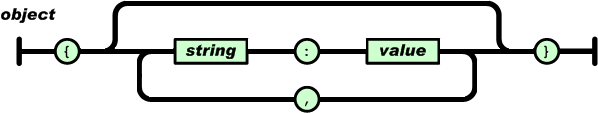
\includegraphics[scale=0.5]{img/json/object.png}
\caption{Objeto JSON}
\end{figure}

Já um \textit{array} é representado utilizando colchete:

\begin{figure}[h]
\centering
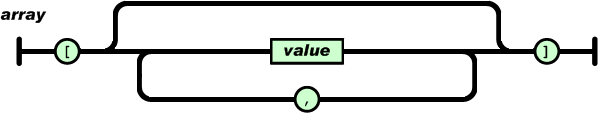
\includegraphics[scale=0.5]{img/json/array.png}
\caption{Array JSON}
\end{figure}

O valor (\textit{value}) pode ser uma \textit{string}, um número, ou \texttt{true} ou \texttt{false},
\texttt{null}, um \textit{array}, ou ainda um objeto. Estas estruturas podem estar aninhadas.

\begin{figure}
\centering
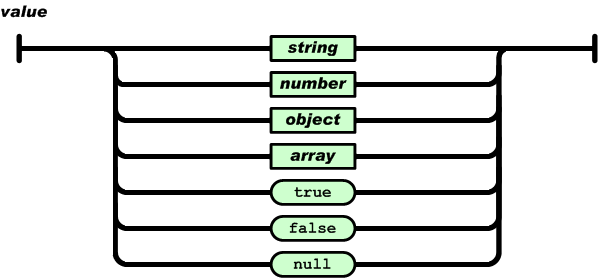
\includegraphics[scale=0.5]{img/json/value.png}
\caption{Possíveis valores}
\end{figure}

Uma \textit{string} é uma coleção de nenhum ou mais caracteres Unicode, envolvido entre aspas duplas usando
barras invertidas como caracter de escape. Um caracter está representando como um simples caracter
de \textit{string}. Uma cadeia de caracteres é parecida com uma cadeia de caracteres em C ou Java.

\begin{figure}
\centering
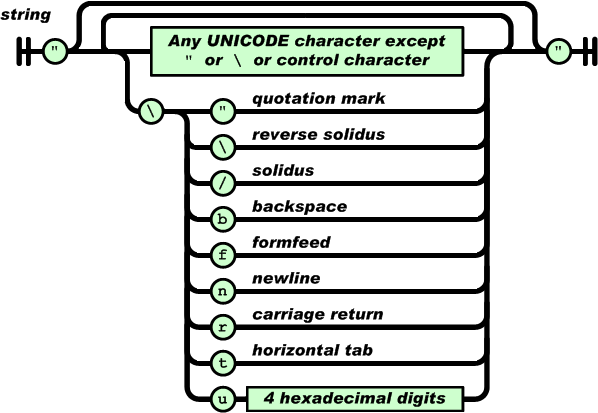
\includegraphics[scale=0.5]{img/json/string.png}
\caption{Formato de uma string}
\end{figure}

Um número é similar a um número em C ou Java, exceto quando não se usa os números octais ou hexadecimais.

\begin{figure}
\centering
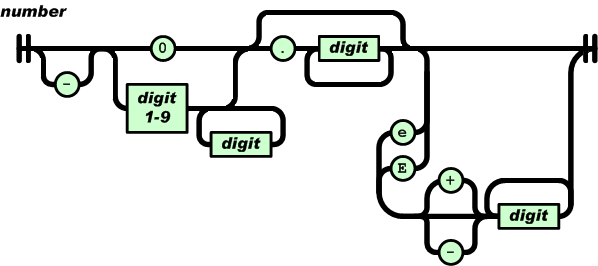
\includegraphics[scale=0.5]{img/json/number.png}
\caption{Formato de um número}
\end{figure}

\subsection*{Exemplo}

Para mostrar como funciona vamos a um exemplo bem prático. Utilizando um browser moderno, como o
chrome/chromium, abra o console que fica em \texttt{Ferramentas $\rightarrow$ Console JavaScript} ou
apenas \texttt{Ctrl + Shift + J}.

% TODO: mostrar exemplo criando um objeto, definindo atributos e imprimindo-os

\printglossary

\end{document}